\chapter{The concept of black hole 1: Horizons as null hypersurfaces}
\label{s:def}

\minitoc

\section{Introduction}

In this chapter, we shall start from a naive ``definition'' of a black hole,
as a region of spacetime from which no particle can escape, and
we shall convince ourselves that the black hole boundary --- the so-called
\emph{event horizon} --- must be a null hypersurface (Sec.~\ref{s:def:BH_null_hypsurf}).
We shall then study the properties of these hypersurfaces
(Secs.~\ref{s:def:geom_null_hypsurf} and \ref{s:def:null_raychaud}).
The precise mathematical definition of a black hole will be given in Chap.~\ref{s:glo}.


%%%%%%%%%%%%%%%%%%%%%%%%%%%%%%%%%%%%%%%%%%%%%%%%%%%%%%%%%%%%%%%%%%%%%%%%%%%%%%%%%%%%%%%%


\section{Black holes and null hypersurfaces} \label{s:def:BH_null_hypsurf}

\subsection{A first definition of black holes} \label{s:def:first_defin}

Given a $n$-dimensional spacetime $(\M,\w{g})$ as presented in Chap.~\ref{s:fra}
(with $n\geq 2$),
a naive definition of a black hole, involving only words, could be
\begin{greybox}
A \defin{black hole}\index{black hole} is a localized region of spacetime
from which neither massive particles nor massless ones (photons) can escape.
\end{greybox}
There are essentially two features in this definition: \emph{localization}
and \emph{inescapability}. Let us for a moment focus on the latter.
It implies the existence of a \emph{boundary}, which no
particle emitted in the black hole region can cross.
This boundary is called the
\defin{event horizon}\index{event!horizon}\index{horizon!event --} and is
quite often referred to simply as the \defin{horizon}.
It is a \defin{one-way membrane}\index{one-way membrane}\index{membrane!one-way --},
in the sense that it can be crossed from the black hole ``exterior'' towards
the black hole ``interior'', but not in the reverse way. The one-way membrane must be
a hypersurface of the spacetime manifold $\M$, for it has to divide $\M$ in two regions:
the interior (the black hole itself) and the exterior region.
Let us recall that a \defin{hypersurface}\index{hypersurface} is an
embedded submanifold of $\M$ of codimension 1
(cf. Sec.~\ref{s:bas:embed} in Appendix~\ref{s:bas}).

\begin{figure}
\centerline{\includegraphics[width=0.45\textwidth]{def_spacelike_hyp.pdf}
\includegraphics[width=0.25\textwidth]{def_timelike_hyp.pdf}
\includegraphics[width=0.30\textwidth]{def_null_hyp.pdf}}
\caption[]{\label{f:def:hypersurfaces} \footnotesize
The three causal types of hypersurfaces:
spacelike (left), timelike (middle) and null (right).}
\end{figure}

\subsection{The event horizon as a null hypersurface} \label{s:def:hor_as_null}

To discuss further which hypersurface could act as a black hole boundary,
one should recall that, on a Lorentzian manifold $(\M,\w{g})$,
a hypersurface $\Sigma$ can locally be classified in three categories.
The classification, called the \defin{causal type}\index{causal!type},
depends on the signature of metric induced by $\w{g}$ on
$\Sigma$  --- the
\defin{induced metric}\index{induced!metric}\index{metric!induced --} being
nothing but the restriction $\left.\w{g}\right| _{\Sigma}$ of $\w{g}$
to vector fields tangent to $\Sigma$.
The hypersurface $\Sigma$ is said to be
\begin{itemize}
\item \defin{spacelike} iff $\left.\w{g}\right| _{\Sigma}$ is positive definite,
i.e. iff $\mathrm{sign} \left.\w{g}\right| _{\Sigma} = (+,\cdots,+)$ ($n-1$ plus signs),
i.e. iff $(\Sigma,  \left.\w{g}\right| _{\Sigma})$ is a Riemannian manifold;
\item \defin{timelike} iff $\left.\w{g}\right| _{\Sigma}$ is a Lorentzian metric,
i.e. iff $\mathrm{sign} \left.\w{g}\right| _{\Sigma} = (-,+,\cdots,+)$ (1 minus sign and
$n-2$ plus signs),
i.e. iff $(\Sigma,  \left.\w{g}\right| _{\Sigma})$ is a Lorentzian manifold;
\item \defin{null} iff $\left.\w{g}\right| _{\Sigma}$ is degenerate\footnote{
Cf. Sec.~\ref{s:bas:metric} in Appendix~\ref{s:bas} for the definition of a
degenerate bilinear form; the degeneracy
implies that the bilinear form $\left.\w{g}\right| _{\Sigma}$ is not,
strictly speaking, a metric on $\Sigma$.}
i.e. iff $\mathrm{sign} \left.\w{g}\right| _{\Sigma} = (0,+,\cdots,+)$
(1 zero and $n-2$ plus signs).
\end{itemize}
All these definitions are local, i.e. apply to a point $p\in\Sigma$.
Of course, it may happen that $\Sigma$ has not the same causal type
among all its points.

The causal type of the hypersurface $\Sigma$
can also be deduced from any normal vector\footnote{
The definition of a vector normal to a hypersurface is recalled in Sec.~\ref{s:bas:hyp_normal} of Appendix~\ref{s:bas}.}
$\w{n}$ to it (cf. Fig.~\ref{f:def:hypersurfaces}):
\begin{itemize}
\item $\Sigma$ spacelike $\iff$ $\w{n}$ timelike;
\item $\Sigma$ timelike $\iff$ $\w{n}$ spacelike;
\item $\Sigma$ null $\iff$ $\w{n}$ null.
\end{itemize}
These equivalences are easily proved by considering a $\w{g}$-orthogonal basis
adapted to $\Sigma$.

\begin{remark}
Null hypersurfaces have the distinctive feature that their normals are
also tangent to them. Indeed, by definition, the normal $\w{n}$ is null iff
$\w{n}\cdot\w{n}=0$, which is nothing but the condition
for $\w{n}$ to be tangent to $\Sigma$.
\end{remark}

\begin{figure}
\centerline{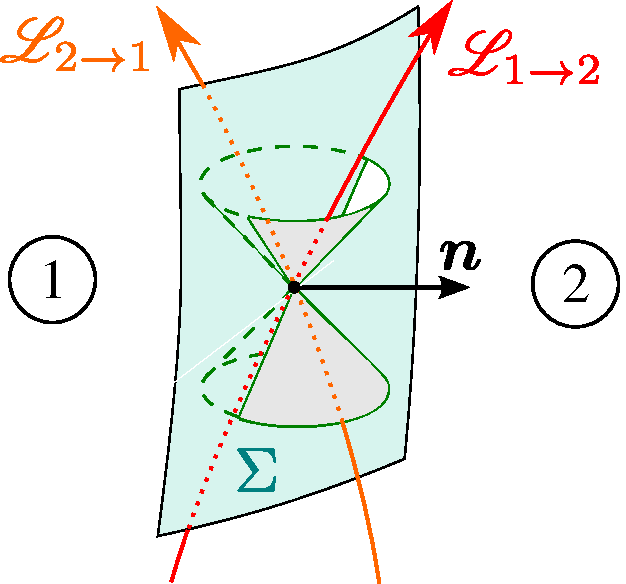
\includegraphics[width=0.4\textwidth]{def_timelike_2way.pdf}}
\caption[]{\label{f:def:timelike_2way} \footnotesize
A timelike hypersurface is a two-way membrane: $\Li_{1\rightarrow 2}$ is
a timelike worldline from Region~1 to Region~2, while $\Li_{2\rightarrow 1}$ is
a timelike worldline from Region~2 to Region~1.}
\end{figure}

\begin{figure}
\centerline{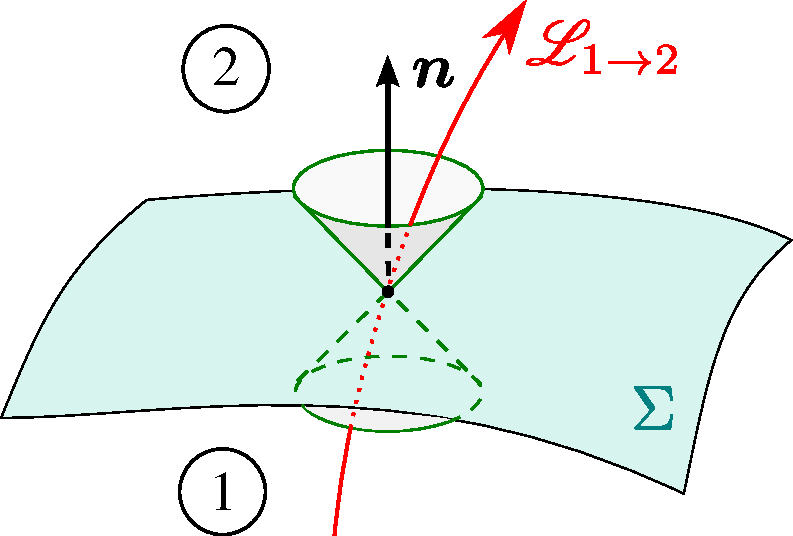
\includegraphics[width=0.5\textwidth]{def_spacelike_1way.pdf}}
\caption[]{\label{f:def:spacelike_1way} \footnotesize
A spacelike hypersurface is a one-way membrane: $\Li_{1\rightarrow 2}$ is
a timelike worldline from Region~1 to Region~2, while there is no timelike or null
worldline from Region~2 to Region~1.}
\end{figure}

\begin{figure}
\centerline{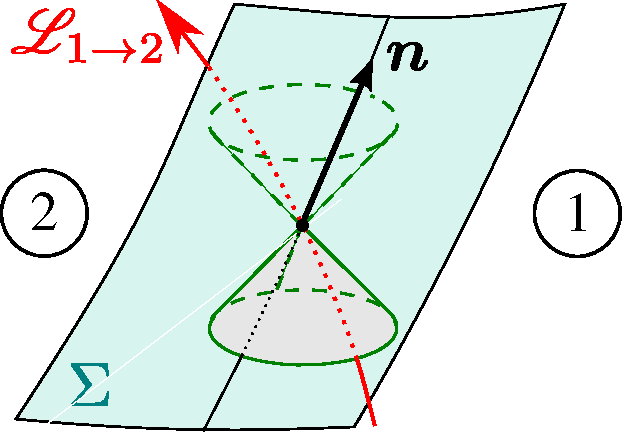
\includegraphics[width=0.5\textwidth]{def_null_1way.pdf}}
\caption[]{\label{f:def:null_1way} \footnotesize
A null hypersurface is a one-way membrane: $\Li_{1\rightarrow 2}$ is
a timelike worldline from Region~1 to Region~2, while there is no timelike or null
worldline from Region~2 to Region~1.}
\end{figure}

A timelike hypersurface is a two-way membrane: it divides (locally)
the spacetime in two regions, 1 and 2 say, and a future-directed timelike or null
worldline can cross it from Region~1 to Region~2, or from Region~2 to Region~1
(see Fig.~\ref{f:def:timelike_2way}). On the contrary,
a spacelike hypersurface is a one-way membrane: a future-directed timelike or null
worldline, which is constrained to move inside the light cones,
can cross it only from Region~1 to Region~2, say (see Fig.~\ref{f:def:spacelike_1way}).
A null hypersurface is also a one-way membrane (see Fig.~\ref{f:def:null_1way}).
At most, a null worldline that is not going from Region~1 to Region~2 must
stay on the hypersurface; an example of such null worldline is
the one depicted in Fig.~\ref{f:def:null_1way} as the thin black line tangent to the normal $\w{n}$.

The limit case between two-way membranes (timelike hypersurfaces)
and one-way ones being null hypersurfaces, it is quite natural to select the
latter ones for the black hole boundary, rather than spacelike hypersurfaces.
This choice will be fully justified in Chap.~\ref{s:glo}, where we shall see
that the generic definition of a black hole implies that its boundary
(the event horizon\index{event!horizon}\index{horizon!event --})
is a null hypersurface as soon as it is smooth (Property~\ref{p:glo:prop4}).
Note however that in Chap.~\ref{s:loc}, we shall see that spacelike hypersurfaces,
called \emph{dynamical
horizons}\index{dynamical!horizon}\index{horizon!dynamical --}, are involved
in quasi-local approaches to black holes.

%%%%%%%%%%%%%%%%%%%%%%%%%%%%%%%%%%%%%%%%%%%%%%%%%%%%%%%%%%%%%%%%%%%%%%%%%%%%%%%%

\section{Geometry of null hypersurfaces} \label{s:def:geom_null_hypsurf}

Since smooth black hole event horizon are null hypersurfaces,
let us examine the geometrical properties of such objects. We shall
denote the hypersurface under study by $\Hor$, for \emph{horizon}, but the results of this section
are valid for any null hypersurface.

\subsection{Hypersurfaces as level sets}

As any hypersurface, $\Hor$ can be locally considered as a \defin{level set}\index{level set}:
around any point of $\Hor$, there exists an open subset $\mathscr{U}$
of $\M$ (possibly  $\mathscr{U} = \M$) and
a smooth scalar field $u:\ \mathscr{U} \rightarrow \R$ such that
\be \label{e:def:Hor_u_zero}
    \forall p \in \mathscr{U},\quad p\in \Hor \iff u(p) = 0
\ee
and
\be \label{e:def:du_not_zero}
    \dd u \not = 0 \quad \mbox{on}\ \Hor ,
\ee
where  $\dd u$ is the \emph{differential} of the scalar field $u$
(cf. Sec.~\ref{s:bas:linear_form}): $\dd u = (\dert{u}{x^\alpha}) \, \dd x^\alpha$
in any coordinate chart $(x^\alpha)$.
Condition (\ref{e:def:du_not_zero}) ensures that $\Hor$ is a regular
hypersurface (an \emph{embedded} submanifold, cf. Sec.~\ref{s:bas:embed}); without it, $\Hor$ could be
self-intersecting.

\begin{figure}
\centerline{\includegraphics[width=0.6\textwidth]{def_null_hplane.pdf}}
\caption[]{\label{f:def:null_hplane} \footnotesize
Null hyperplane $\Hor$ of equation $t-x=0$ in Minkowski spacetime.
The dimension along $z$ has been suppressed, so that $\Hor$ is pictured as a
2-plane.}
\end{figure}


\begin{example}[null hyperplane] \label{x:def:null_hyp}
A very simple example of null hypersurface is a null hyperplane of
the 4-dimensional Minkowski spacetime. The \defin{Minkowski spacetime}\index{Minkowski!spacetime} is defined by $\M=\mathbb{R}^4$ with $\w{g}$ being a \emph{flat} Lorentzian
metric. Natural coordinates are \defin{Minkowskian coordinates}\index{Minkowskian coordinates} $(t,x,y,z)$,
i.e. coordinates with
respect to which the metric components are $g_{\alpha\beta} = \mathrm{diag}(-1,1,1,1)$. The scalar field
\be \label{e:def:null_plane_u}
    u(t,x,y,z) = t - x
\ee
defines then a null hyperplane $\Hor$ by $u=0$ (cf. Fig.~\ref{f:def:null_hplane}).
\end{example}

\begin{example}[light cone] \label{x:def:light_cone}
Another simple example of null hypersurface, still in the 4-dimensional Minkowski spacetime,
is the future sheet $\Hor$ of a light cone\index{light!cone}\index{cone!light --}, also
called \defin{future light cone}\index{future!light cone}. Note that we have
to take out the cone apex from $\Hor$, in order to have a regular hypersurface.
In the  Minkowskian coordinates $(t,x,y,z)$, the choice of the
``retarded time''\index{retarded!time}
\be \label{e:def:light_cone_u}
    u(t,x,y,z) = t - \sqrt{x^2+y^2+z^2}
\ee
defines a future light cone $\Hor$ by $u=0$ and $t>0$ (cf.
Fig.~\ref{f:def:future_light_cone}).
\end{example}

\begin{figure}
\centerline{\includegraphics[width=0.6\textwidth]{def_future_light_cone.pdf}}
\caption[]{\label{f:def:future_light_cone} \footnotesize
Future sheet $\Hor$ of the light cone of equation $t-\sqrt{x^2+y^2+z^2}=0$ in Minkowski spacetime.
The dimension along $z$ has been suppressed, so that $\Hor$ looks 2-dimensional,
whereas it is actually 3-dimensional.}
\end{figure}


\begin{example}[Schwarzschild horizon] \label{x:def:Schw_hor}
Let us consider the 4-dimensional spacetime $(\M,\w{g})$ with $\M$ diffeomorphic
to $\mathbb{R}^4$ and equipped with a coordinate system $(x^\alpha)=(t,r,\th,\ph)$
($t\in \mathbb{R}$, $r\in(0,+\infty)$, $\th\in(0,\pi)$
and $\ph\in(0,2\pi)$) such that the metric tensor takes the
form\footnote{Formula (\ref{e:def:Schw_metric}) follows the notation
introduced in Eq.~(\ref{e:fra:g_components_dx}); see Sec.~\ref{s:bas:metric}
in Appendix~\ref{s:bas} for an extended discussion, in particular Eq.~(\ref{e:bas:sym_tensor_prod}).
When reading the metric components $(g_{\alpha\beta})$ from (\ref{e:def:Schw_metric}), keep in mind that
cross terms involve a factor $2$: the $4m/r$ coefficient of $\dd t \, \dd r$ implies
that $g_{tr} = 2m/r$.}
\be \label{e:def:Schw_metric}
    \w{g} = - \left( 1 - \frac{2 m}{r} \right) \dd t^2
        + \frac{4m}{r} \, \dd t \, \dd r
        + \left( 1 + \frac{2 m}{r} \right) \dd r^2
        + r^2\dd\th^2 + r^2\sin^2\th \, \dd\ph^2 ,
\ee
where $m$ is a positive constant. We shall see in Chap.~\ref{s:sch} that
$(\M,\w{g})$ is actually a part of Schwarzschild spacetime\index{Schwarzschild!spacetime}, described in
coordinates different from the standard Schwarzschild-Droste ones,  $(\bar t, r, \th, \ph)$
say, the link between the two being
$t = {\bar t} + 2m\ln|r/(2m)-1|$. The present coordinates are called the
\defin{ingoing Eddington-Finkelstein coordinates}\index{Eddington-Finkelstein!coordinates}
and have the advantage over the standard ones to be regular on the event horizon,
which is located at $r=2m$. Indeed, the metric components (\ref{e:def:Schw_metric})
remain finite when $r\rightarrow 2m$, as those of the inverse metric, which are
\be \label{e:def:Schw_metric_inv}
    g^{\alpha\beta} = \left(
    \begin{array}{cccc}
    - \left( 1 + \frac{2m}{r} \right) & \frac{2m}{r} & 0 & 0 \\
    \frac{2m}{r} & 1 - \frac{2m}{r} & 0 & 0 \\
    0 & 0 & \frac{1}{r^2} & 0 \\
    0 & 0 & 0 & \frac{1}{r^2\sin^2\th}
    \end{array} \right) .
\ee
Let us consider the scalar field defined on $\M$ by
\be \label{e:def:Schw_u}
    u(t,r,\th,\ph) = \left( 1 - \frac{r}{2m} \right)
            \exp\left(\frac{r-t}{4m}\right) .
\ee
It is then clear that the hypersurface $u=0$ is the
3-dimensional ``cylinder'' $\Hor$ of equation
$r=2m$ (cf. Fig.~\ref{f:def:Schwarz_horizon}). We shall see below\footnote{This should be obvious to the experienced
reader, since a normal 1-form to $\Hor$ is $\dd r$ and
from Eq.~(\ref{e:def:Schw_metric_inv}), $g^{\mu\nu} \partial_\mu r \, \partial_\nu r = g^{rr}=0$ on $\Hor$.} that $\Hor$ is indeed a null hypersurface.
\end{example}

\begin{figure}
\centerline{\includegraphics[width=0.5\textwidth]{def_Schwarz_horizon.pdf}}
\caption[]{\label{f:def:Schwarz_horizon} \footnotesize
Schwarzschild horizon $\Hor$ introduced in Example~\ref{x:def:Schw_hor};
The figure is drawn for $\th=\pi/2$ and is based on coordinates $(t,x,y)$
related to the ingoing Eddington-Finkelstein coordinates $(t,r,\th,\ph)$
by $x=r\cos\ph$ and $y=r\sin\ph$.}
\end{figure}



\subsection{Null normals} \label{s:def:null_normal}

Let $\wl$ be a vector field normal to $\Hor$. Since $\Hor$ is a null hypersurface,
$\wl$ is a null vector:
\be \label{e:def:wl_null}
    \wl\cdot\wl = 0 .
\ee
Moreover, we choose $\wl$ to be future-directed (cf. Sec.~\ref{s:fra:time_orientation}).

\begin{remark}
As a consequence of (\ref{e:def:wl_null}), there is no natural normalization
of $\wl$, contrary to the case of timelike or spacelike hypersurfaces,
where one can always choose the normal to be a unit vector
(scalar square equal to $1$ or $-1$). It follows that there is no unique choice
of $\wl$. At this stage, any rescaling $\wl \mapsto \wl' =  \alpha \wl$, with
$\alpha$ some strictly positive (to preserve the future orientation of $\wl$)
scalar field on $\Hor$,
yields a normal vector field $\wl'$ as valid as $\wl$.
\end{remark}
The null normal vector field $\wl$ is a priori defined on $\Hor$
only and not at points $p\not\in\Hor$.
However, it is worth to consider $\wl$ as a vector field
not confined to $\Hor$ but defined
in some open subset of $\M$ around $\Hor$.
In particular this would permit to define the spacetime covariant
derivative $\w{\nabla}\wl$, which is not possible if the
support of $\wl$ is restricted to $\Hor$.
Following Carter \cite{Carte97}, a simple way to achieve
this is to consider not only a single null hypersurface $\Hor$,
but a foliation of $\M$ (in the vicinity
of $\Hor$) by a family of null hypersurfaces, such that $\Hor$ is an
element of this family.
Without any loss of generality,
we may select the value of the scalar field $u$ defining $\Hor$ to label these hypersurfaces and
denote the family by $(\Hor_u)$. The null hypersurface $\Hor$
is then nothing but the element $\Hor = \Hor_{u=0}$ of this family
[Eq.~(\ref{e:def:Hor_u_zero})].
The vector field $\wl$ can then be viewed as being defined in the part of $\M$
foliated by $(\Hor_u)$, such that at each point in this region, $\wl$
is null and normal to $\Hor_u$ for some value of $u$.

\begin{figure}
\centerline{\includegraphics[height=0.4\textheight]{def_Schwarz_Hu.pdf}}
\caption[]{\label{f:def:Schwarz_Hu} \footnotesize
Hypersurfaces $\Hor_u$ defined by $u=\mathrm{const}$ for
the Schwarzschild horizon (Example~\ref{x:def:Schw_hor}).}
\end{figure}



\begin{example}
The scalar field $u$ introduced in Example~\ref{x:def:null_hyp}
(null hyperplane) does define a family of null hypersurfaces
$(\Hor_u)$. A counter-example would be $u(t,x,y,z)=(t-x)(1+x^2)$, since
$u=a$ does not define a null hypersurface except for $a=0$.
Similarly, the scalar fields $u$ of
Example~\ref{x:def:light_cone} (light cone)
and Example~\ref{x:def:Schw_hor} (Schwarzschild horizon)
do define a family of null
hypersurfaces $(\Hor_u)$.
In the latter example, this would not have been the
case for the simpler choice $u(t,r,\th,\ph)  = r - 2m$.
Some of these null hypersurfaces are represented in Fig.~\ref{f:def:Schwarz_Hu}
\end{example}

Obviously the family $(\Hor_u)$ is non-unique but all geometrical
quantities that we shall introduce hereafter do not depend upon the choice
of the foliation $\Hor_u$ once they are evaluated at $\Hor$.

Since $\Hor$ is a hypersurface where $u$ is constant [Eq.~(\ref{e:def:Hor_u_zero})],
we have, by definition,
\be
    \forall \w{v}\in T_p\M,\quad \w{v} \mbox{\ tangent to\ }\Hor
    \iff  \wnab_{\w{v}}\,  u = 0
    \iff  \langle \dd u , \w{v} \rangle = 0
    \iff  \vw{\nabla} u \cdot \w{v} = 0 ,   \label{e:def:nab_u_normal}
\ee
where $\vw{\nabla} u$ is the \defin{gradient}\index{gradient} of the scalar field $u$,
i.e. the vector field that is the metric-dual of the 1-form $\dd u$
(cf. Sec.~\ref{s:bas:metric_dual});
in a coordinate chart $(x^\alpha)$, its components are given by
\be \label{e:def:nab_up_u}
    \nabla^\alpha u = g^{\alpha\mu} \nabla_{\mu} u = g^{\alpha\mu} \der{u}{x^\mu} .
\ee
Property (\ref{e:def:nab_u_normal}) means that $\vw{\nabla} u$ is
a normal vector field to $\Hor$. By uniqueness of the normal direction to a hypersurface, it
must then be collinear to $\wl$. Therefore, there must exist some scalar
field $\rho$ such that
\be \label{e:def:wl_rho_u}
    \encadre{\wl = - \mathrm{e}^\rho \, \vw{\nabla} u } .
\ee
We have chosen the
coefficient linking $\wl$ and $\vw{\nabla} u $ to be strictly negative
(minus an exponential). This is always possible by a suitable
choice of the scalar field $u$. The minus sign ensures that in the case
of $u$ increasing toward the future, $\wl$ is future-directed,
as the following example shows:

\begin{example}[null hyperplane] \label{x:def:null_hyp2}
We deduce from
expression (\ref{e:def:null_plane_u}) for $u$ in Example~\ref{x:def:null_hyp} that
$\dd u = \dd t - \dd x$.
The gradient vector field obtained by metric duality is
$\vw{\nabla} u = - \wpar_t - \wpar_x$. Choosing for simplicity $\rho=0$,
formula~(\ref{e:def:wl_rho_u}) yields
\be \label{e:def:wl_null_hyperplane}
    \wl =  \wpar_t + \wpar_x .
\ee
This vector field is depicted in Fig.~\ref{f:def:null_hplane}.
\end{example}

\begin{example}[light cone] \label{x:def:light_cone2}
Regarding Example~\ref{x:def:light_cone}, we have,
given expression (\ref{e:def:light_cone_u}) for $u$,
\[
    \dd u = \dd t - \frac{x}{r} \dd x - \frac{y}{r} \dd y - \frac{z}{r} \dd z,
    \quad\mbox{with}\quad r:=\sqrt{x^2+y^2+z^2}.
\]
Choosing for simplicity $\rho=0$ in (\ref{e:def:wl_rho_u}), we get the
normal
\be \label{e:def:wl_light_cone}
    \wl = \wpar_t + \frac{x}{r} \wpar_x + \frac{y}{r} \wpar_y + \frac{z}{r} \wpar_z .
\ee
This vector field is depicted in Fig.~\ref{f:def:future_light_cone}.
\end{example}

\begin{example}[Schwarzschild horizon] \label{x:def:Schw_hor2}
We deduce from expression (\ref{e:def:Schw_u}) for $u$ in
Example~\ref{x:def:Schw_hor} that
\[
    \dd u = \frac{1}{4 m} \mathrm{e}^{(r-t)/(4m)} \left[ - \left(1-\frac{r}{2m}  \right)
        \, \dd t
        - \left(1 + \frac{r}{2m}\right) \, \dd r \right] .
\]
The corresponding gradient vector field,
is computed from (\ref{e:def:nab_up_u}) via expression
(\ref{e:def:Schw_metric_inv}) for $g^{\alpha\mu}$:
\[
    \vw{\nabla} u = \frac{1}{4 m} \mathrm{e}^{(r-t)/(4m)} \left[
    - \left(1+ \frac{r}{2m} \right) \wpar_t
    + \left(1 - \frac{r}{2m} \right) \wpar_r \right] .
\]
This time, we do not chose $\rho=0$ but rather select $\rho$ so that
$\el^t = 1$:
\be \label{e:def:rho_Schw_hor}
    \mathrm{e}^\rho =  - \frac{1}{\nabla^t u} \iff
    \rho = \frac{t-r}{4m} - \ln \left( 1 + \frac{r}{2m} \right) + \ln (4 m).
\ee
Equation~(\ref{e:def:wl_rho_u}) leads then to
\be \label{e:def:wl_Schw_hor}
    \wl = \wpar_t +  \frac{r-2m}{r+2m} \,  \wpar_r .
\ee
Given the metric (\ref{e:def:Schw_metric}), we check that $\w{g}(\wl, \wl)=0$.
Since $\wl\not=0$, this proves that all hypersurfaces $\Hor_u$, and in particular $\Hor$,
are null.
The vector field $\wl$ is depicted on $\Hor$ in Fig.~\ref{f:def:Schwarz_horizon}
and in all $\M$ in Fig.~\ref{f:def:Schw_hor_lk}.
\end{example}

\subsection{Null geodesic generators} \label{s:def:null_geod_gen}

\subsubsection{Frobenius identity} \label{s:def:Frobenius}

Let us take the metric dual of Eq.~(\ref{e:def:wl_rho_u}); it writes
$\uu{\el} = - \mathrm{e}^\rho \, \dd u = - \mathrm{e}^\rho \, \wnab u $, or, in index notation,
$\el_\alpha = - \mathrm{e}^\rho \, \nabla_\alpha u$.
Taking the covariant derivative, we get
\[
    \nabla_\alpha \el_\beta = - \mathrm{e}^\rho \nabla_\alpha \rho \nabla_\beta u
                -   \mathrm{e}^\rho  \nabla_\alpha \nabla_\beta u
                 = \nabla_\alpha \rho \, \el_\beta - \mathrm{e}^\rho  \nabla_\alpha \nabla_\beta u
\]
Antisymmetrizing and using the torsion-free property of $\wnab$ (i.e.
$\nabla_\alpha \nabla_\beta u - \nabla_\beta \nabla_\alpha u = 0$, cf.
Eq.~(\ref{e:bas:torsion-free})), we get
\be \label{e:def:ext_der_wl_comp}
  \nabla_\alpha \el_\beta - \nabla_\beta \el_\alpha =
  \nabla_\alpha \rho \, \el_\beta -  \nabla_\beta \rho \, \el_\alpha  .
\ee
In the left-hand side there appears the exterior derivative $\dd\uu{\el}$ of
the 1-form $\uu{\el}$ [cf. Eq.~(\ref{e:bas:def_ext_1f_nab})],
while one recognizes in the right-hand side the exterior product of
the two 1-forms $\dd\rho$ and $\uu{\el}$. Hence we may rewrite (\ref{e:def:ext_der_wl_comp})
as
\be
    \encadre{ \dd \uu{\el} = \dd\rho \wedge \uu{\el} } .
\ee
This reflects the \defin{Frobenius theorem}\index{Frobenius!theorem}
in its dual formulation (see e.g.
Theorem B.3.2 in Wald's textbook \cite{Wald84} or Theorem C.2 in
Straumann's textbook \cite{Strau13}):
the exterior derivative of
the 1-form $\uu{\el}$ is the exterior product of
some 1-form (here $\dd\rho$) with $\uu{\el}$ itself if, and only if,
$\uu{\el}$ defines hyperplanes that are integrable in some hypersurface ($\Hor$ in the present case).

\subsubsection{Geodesic generators} \label{s:def:geod_gener}

Let us contract the Frobenius identity (\ref{e:def:ext_der_wl_comp}) with $\wl$:
\be \label{e:def:l_contract_Frob}
    \el^\mu \nabla_\mu \el_\alpha - \el^\mu \nabla_\alpha \el_\mu
        = \el^\mu \nabla_\mu \rho \, \el_\alpha
        - \underbrace{\el^\mu \el_\mu}_{0} \nabla_\alpha \rho .
\ee
Now, since $\wl$ is a null vector,
$\el^\mu \nabla_\alpha \el_\mu = \nabla_\alpha (\el^\mu \el_\mu)
        - \el_\mu \nabla_\alpha \el^\mu = - \el_\mu \nabla_\alpha \el^\mu$,
from which we get
\be \label{e:def:el_nab_el_zero}
    \el^\mu \nabla_\alpha \el_\mu = 0 .
\ee
Hence (\ref{e:def:l_contract_Frob}) reduces to
\be \label{e:def:wl_geod_kappa_dual}
    \el^\mu \nabla_\mu \el_\alpha  = \kappa \, \el_\alpha ,
\ee
with
\be \label{e:def:def_kappa}
    \kappa := \el^\mu \nabla_\mu \rho = \wnab_{\wl}\,  \rho .
\ee
The metric dual of (\ref{e:def:wl_geod_kappa_dual}) is
\be \label{e:def:wl_geod_kappa}
    \encadre{ \wnab_{\wl}\, \wl = \kappa \, \wl } .
\ee
This equation implies that the field lines of $\wl$ are geodesics
(cf. Appendix~\ref{s:geo}).
To demonstrate this, we note that a rescaling
\be \label{e:def:wl_rescale}
    \wl \mapsto \wl' =  \alpha \wl
\ee
with $\alpha$ a positive scalar field can be performed to yield
a \defin{geodesic vector field}\index{geodesic!vector field} $\wl'$, i.e.
a vector field that obeys\footnote{A vector field that obeys the weaker condition
(\ref{e:def:wl_geod_kappa}), with $\kappa$ possibly different from zero, is called
a \defin{pregeodesic vector field}\index{pregeodesic!vector field}, cf.
Sec.~\ref{s:geo:gener_param}.} Eq.~(\ref{e:geo:geod_eq_v}):
\be \label{e:def:wlp_geod}
    \wnab_{\wl'}\, \wl' = 0 .
\ee
\begin{proof}
Equations~(\ref{e:def:wl_rescale}) and
(\ref{e:def:wl_geod_kappa}) imply
\be \label{e:def:nab_lp_lp}
    \wnab_{\wl'}\, \wl' = \alpha\left(
        \wnab_{\wl}\, \alpha + \kappa \alpha \right) \wl .
\ee
Hence, since $\alpha>0$,
\[
    \wnab_{\wl'}\, \wl' = 0  \iff  \wnab_{\wl}\, \ln \alpha = -\kappa
    \iff \derd{}{\lambda} \ln \alpha = - \kappa ,
\]
where $\lambda$ is the parameter associated to $\wl$ along its field lines $\Li$:
$\wl = \left. \D\w{x}/\D\lambda \right| _\Li$.
Therefore, setting $\alpha(\lambda) = \exp(- \int_0^\lambda \kappa(\lambda') \D\lambda')$
along each field line $\Li$
ensures that $\wl' = \alpha\wl$ fulfills Eq.~(\ref{e:def:wlp_geod}).
\end{proof}

Because of (\ref{e:def:wlp_geod}),
the field lines of $\wl'$ are  null geodesics and $\wl'$ is the tangent
vector to them associated with some \emph{affine} parameter $\lambda'$.
On the other side, if $\kappa\not=0$, $\wl$ is not a geodesic vector field
and therefore cannot be associated with some affine parameter. For this
reason the quantity $\kappa$ is called the
\defin{non-affinity coefficient}\index{non-affinity coefficient} of
the null normal $\wl$ (cf. Sec.~\ref{s:geo:gener_param} in Appendix~\ref{s:geo}).

Since $\wl$ is collinear to $\wl'$, it obviously shares the same field lines,
which have just been shown to be null geodesics. Hence we may state:

\begin{prop}[geodesic generators of a null hypersurface]
\label{p:def:null_geod_generators}
Any null hypersurface $\Hor$ is ruled by a family of null geodesics, called the
\defin{null geodesic generators}\index{null!geodesic!generator}\index{generator!of a null hypersurface} of $\Hor$, and each vector field $\wl$ normal to $\Hor$ is
tangent to these null geodesics.
\end{prop}

\begin{remark}
\label{r:def:null_curves}
The above result is not trivial: while it is obvious that the field lines of the normal
vector field $\wl$ are null curves that are tangent to $\Hor$, one must
keep in mind that not all null curves are null geodesics. For instance, in
Minkowski spacetime, the helix defined in terms of
some Minkowskian coordinates $(x^\alpha)=(t,x,y,z)$ by the parametric equation
$x^\alpha(\lambda) = (\lambda, \cos\lambda, \sin\lambda, 0)$ is a null curve, i.e.
it has
a null tangent vector at each point, but it is not a null geodesic: in Minkowski
spacetime, all null geodesics are straight lines.
\end{remark}

As a by-product of Eq.~(\ref{e:def:nab_lp_lp}), we get the behaviour of the
non-affinity coefficient under a rescaling of the null normal:
\be \label{e:def:rescale_kappa}
    \wl' = \alpha \wl \ \Longrightarrow \ \kappa' = \alpha \kappa + \wnab_{\wl} \alpha .
\ee

\begin{example}[null hyperplane] \label{x:def:null_hyp3}
It is clear on expression (\ref{e:def:wl_null_hyperplane}) for $\wl$ that
the covariant derivative
$\wnab \wl$ vanishes identically. In particular $\wnab_{\wl} \wl = 0$.
Equation~(\ref{e:def:wl_geod_kappa}) then implies $\kappa = 0$,
which is in agreement with Eq.~(\ref{e:def:def_kappa}) and the choice $\rho=0$
performed in Example~\ref{x:def:null_hyp2}. The null geodesic generators of $\Hor$ are the
straight lines defined by $t=x$, $y=y_0$ and $z=z_0$ for some constants
$(y_0,z_0)\in \mathbb{R}^2$.
They are depicted as green lines in Fig.~\ref{f:def:null_hplane}.
 Either $t$ or $x$ can be chosen as affine
parameters of these generators.
\end{example}

\begin{example}[light cone] \label{x:def:light_cone3}
From expression (\ref{e:def:wl_light_cone})
for $\wl$ and the fact that
$\nabla_\beta \el^\alpha = \partial_\beta \el^\alpha$
in the Minkowskian coordinates $(t,x,y,z)$, we get
\be \label{e:def:nab_l_light_cone}
    \nabla_\beta \el^\alpha = \left(
    \begin{array}{cccc}
    0 & 0 & 0 & 0 \\
    0 & \frac{y^2+z^2}{r^3} & - \frac{xy}{r^3} & - \frac{xz}{r^3} \\
    0 & - \frac{xy}{r^3} & \frac{x^2+z^2}{r^3} & - \frac{yz}{r^3} \\
    0 & - \frac{xz}{r^3} & - \frac{yz}{r^3} & \frac{x^2+y^2}{r^3}
    \end{array} \right)
    \qquad {(\alpha = \mbox{row index}; \atop \beta = \mbox{column index}).}
\ee
We obtain then $\el^\mu \nabla_\mu \el^\alpha = 0$.
From Eq.~(\ref{e:def:wl_geod_kappa}), we conclude that $\kappa = 0$,
which is in agreement with Eq.~(\ref{e:def:def_kappa}) and the choice $\rho=0$
performed in Example~\ref{x:def:light_cone2}. The null geodesic generators of $\Hor$
are the half-lines defined by $x=a t$, $y=b t$, $z = \sqrt{1-a^2-b^2} t$, with
$t>0$ and $(a,b)\in\mathbb{R}^2$ such that $a^2+b^2 \leq 1$.
They are depicted as green lines in Fig.~\ref{f:def:future_light_cone}.
Since from (\ref{e:def:wl_light_cone}) $\wnab_{\wl} t = 1$
and $\kappa=0$, $\lambda=t$ is an affine parameter along these null geodesic generators.
\end{example}

\begin{example}[Schwarzschild horizon] \label{x:def:Schw_hor3}
The covariant derivative of the vector field $\wl$ as given by (\ref{e:def:wl_Schw_hor})
is (cf. Sec.~\ref{s:sam:Schwarz_hor} for the computation)
\be \label{e:def:nab_l_Schw_hor}
    \nabla_\beta \el^\alpha = \left(
    \begin{array}{cccc}
    \frac{m}{r^2} & \frac{m}{r^2} \frac{3r+2m}{r+2m} & 0 & 0 \\[1ex]
    \frac{m}{r^2}\frac{r-2m}{r+2m} & \frac{m}{r^2}\frac{3r^2-4m(r+m)}{(r+2m)^2} & 0 & 0 \\[1ex]
    0 & 0 & \frac{r-2m}{r(r+2m)} & 0 \\
    0 & 0 & 0 & \frac{r-2m}{r(r+2m)}
    \end{array} \right)
    \qquad {(\alpha = \mbox{row index}; \atop \beta = \mbox{column index}).}
\ee
Contracting with $\wl^\beta$, we obtain
\[
    \wnab_{\wl} \wl = \frac{4m}{(r+2m)^2} \wpar_t
        +  \frac{4m(r-2m)}{(r+2m)^3} \,  \wpar_r = \frac{4m}{(r+2m)^2}  \, \wl .
\]
Hence, for any $\Hor_u$, $\kappa=4m/(r+2m)^2$. On $\Hor$ ($r=2m$), we get
\be \label{e:def:kappa_Schw_hor}
   \kappa = \frac{1}{4m} .
\ee
This value agrees with $\kappa = \wnab_{\wl}\rho$ [Eq.~(\ref{e:def:def_kappa})] and the
choice (\ref{e:def:rho_Schw_hor}) made for $\rho$. Contrary to Examples~\ref{x:def:null_hyp3}
and \ref{x:def:light_cone3}, $\kappa$ does not vanish; hence $t$, which is
a parameter of the null geodesic generators associated with $\wl$ (since $\wnab_{\wl} t = 1$
by virtue of (\ref{e:def:wl_Schw_hor})),
is \emph{not} an affine parameter. The null geodesic generators are depicted
as vertical green lines in Fig.~\ref{f:def:Schwarz_horizon}.
\end{example}

\subsection{Cross-sections} \label{s:def:spacelike_sections}

Let us now focus on the first aspect of the black hole definition given
in Sec.~\ref{s:def:first_defin}: \emph{localization}.
This feature is crucial to distinguish a black hole boundary from other kinds
of null hypersurfaces. For instance the interior of a future null cone
in Minkowski spacetime is a region from which no particle may escape,
but since the null cone is expanding indefinitely, particles can travel arbitrary far from
the center. Therefore, a null cone does not define a black hole.
A key parameter is hence the \emph{expansion} of null hypersurfaces, which we shall
discuss in the next section, after having introduced cross-sections.

\begin{greybox}
Let $\Hor$ be a null hypersurface of a $n$-dimensional spacetime $(\M, \w{g})$
with $n\geq 3$.
We define a \defin{cross-section}\index{cross-section} of $\Hor$
as a submanifold $\Sp$ of $\Hor$ of dimension $n-2$
such that (i) the null normal $\wl$ is nowhere tangent to $\Sp$ and (ii)
each null geodesic generator of $\Hor$ intersects $\Sp$ at most once.
If each null geodesic generator intersects $\Sp$ exactly once,
we shall say that $\Sp$ is a
\defin{complete cross-section}\index{cross-section!complete --}\index{complete!cross-section}
(cf. Fig.~\ref{f:def:hor_cylinder}).
\end{greybox}

\begin{figure}
\centerline{\includegraphics[width=0.5\textwidth]{def_cross_sections.pdf}}
\caption[]{\label{f:def:hor_cylinder} \footnotesize
The null hypersurface $\Hor$ and two (complete) cross-sections $\Sp$ and $\Sp'$.
The green curves represent some null geodesic generators, with the null normal
$\wl$ tangent to them.}
\end{figure}

\begin{notation}
Indices relative to a cross-section will range from $2$ to $n-1$ and
will be denoted by a Latin letter from the beginning of the alphabet: $a$, $b$, etc.
\end{notation}

To encompass the idea that an event horizon $\Hor$ delimitates some
region of spacetime, we shall assume that its cross-sections
are \defin{closed manifolds}\index{closed!manifold}, i.e.
are compact without boundary\footnote{Scrictly speaking, a
\emph{closed manifold} is simply a \emph{compact manifold},
since a topological manifold, as defined in Sec.~\ref{s:bas:def_manif},
has no boundary. Indeed, the concept of \emph{manifold with boundary} requires
a separate definition (cf. Sec.~\ref{s:bas:manif_boundary}),
so that a manifold with boundary is not a manifold.
Hence, we may consider the terminology \emph{closed manifold}
as stressing the no-boundary aspect of a compact manifold.}.
The simplest example is the sphere,
more precisely the $(n-2)$-dimensional sphere $\mathbb{S}^{n-2}$,
as illustrated in Fig.~\ref{f:def:hor_cylinder}.
This example is the one relevant for standard 4-dimensional
stationary black holes, thanks a topology theorem that
we shall discuss in Sec.~\ref{s:sta:BH_stationary}.
But for $n > 4$, other
compact topologies, like that of a torus, are allowed for
cross-sections of a stationary black hole.

A first important property of cross-sections, independently whether it is closed or not,
is:
\begin{prop}[spacelike character of cross-sections]
\label{p:def:spacelike_cs}
Any cross-section $\Sp$ of a null hypersurface is spacelike,
i.e. all vectors tangent to $\Sp$ are spacelike.
\end{prop}
The spacelike character of $\Sp$ follows from
\begin{lemma}[tangent vectors to a null hypersurface]
\label{p:def:tangent_to_null_hyp}
Every nonzero tangent vector $\w{v}$ to a null hypersurface is either spacelike or null.
Moreover, if it is null, $\w{v}$ is tangent to a null geodesic generator, i.e. $\w{v}$ is normal
to the hypersurface.
\end{lemma}
\begin{proof}
Tangent vectors to a null hypersurface $\Hor$ are by definition
vectors $\w{v}$ such that $\w{g}(\wl,\w{v})=0$, where $\wl$ is the normal
to $\Hor$. Since $\wl$ is null, it follows then from Property~\ref{p:fra:corol1}
(Sec.~\ref{s:fra:time_orientation}) that $\w{v}$ cannot be timelike.
Besides, if $\w{v}$ is null, Property~\ref{p:fra:corol2} (Sec.~\ref{s:fra:time_orientation})
implies that it must be collinear to $\wl$.
\end{proof}
\begin{proof}[Proof of Property~\ref{p:def:spacelike_cs}]
Let $p \in \Sp$ and $\w{v}\in T_p\M$ be a nonzero vector tangent to $\Sp$.
The above lemma implies that $\w{v}$ is either spacelike or tangent to the
null geodesic generator $\Li$ going through $p$, but then $\Li$ would be tangent to $\Sp$,
which is not allowed, given the definition of a cross-section. We conclude
that $\w{v}$ is necessarily spacelike, which proves that $\Sp$ is a spacelike
submanifold.
\end{proof}

\begin{example}[light cone] \label{x:def:light_cone4}
The future sheet $\Hor$ of the Minkowski-spacetime light cone considered in
Examples~\ref{x:def:light_cone},
\ref{x:def:light_cone2} and \ref{x:def:light_cone3} has the topology $\R \times \SS^2$
since we have excluded the cone apex from $\Hor$.
The complete cross-sections are then compact and it natural to choose them as the
spheres defined by $t=t_0$ for some positive constant $t_0$:
$\Sp = \left\{ p \in \Hor,\  t(p) = t_0 \right\}$.
That $\Sp$ is a 2-dimensional sphere in the hyperplane $t=t_0$ is clear on its equation in terms
of the Minkowskian coordinates $(t,x,y,z)$:
\[
\Sp: \quad t=t_0 \quad\mbox{and}\quad x^2+y^2+z^2 = t_0^2,
\]
which follows immediately from $u=0$
[cf. Eq.~(\ref{e:def:light_cone_u})]. Moreover, this equation shows that the
radius of the sphere is $t_0$.
\end{example}

\begin{example}[Schwarzschild horizon] \label{x:def:Schw_hor4}
The 3-dimensional cylinder $\Hor$ introduced in Example~\ref{x:def:Schw_hor}
has the topology $\R \times \SS^2$
(cf. Fig.~\ref{f:def:Schwarz_horizon}).
Since it is defined
by $r=2m$ in terms of the ingoing Eddington-Finkelstein coordinates $(t,r,\th,\ph)$,
a natural coordinate system on $\Hor$ is $x^A = (t,\th,\ph)$. Moreover, we
have seen that the coordinate $t$ is the (non-affine) parameter of the null
geodesics generating $\Hor$ associated with the null normal $\wl$.
As in Example~\ref{x:def:light_cone4}, a natural choice of cross-section is a
sphere defined by $t=t_0$ for some constant $t_0$:
$\Sp = \left\{ p \in \Hor,\  t(p) = t_0 \right\}$.
The equation of $\Sp$ in terms of the coordinates $(t,r,\th,\ph)$ is then
\[
    \Sp: \quad t=t_0 \quad\mbox{and}\quad r = 2m .
\]
Note that $x^a=(\th,\ph)$ constitutes a coordinate system on $\Sp$.
\end{example}

\begin{example}[binary black hole]
Some cross-sections of the event horizon $\Hor$ in numerically
generated binary black hole spacetimes are displayed in Figs.~\ref{f:glo:EH_headon}
and \ref{f:glo:EH_binspir} of Chap.~\ref{s:glo}.
\end{example}

Let us denote by $\w{q}$ the
\defin{metric induced by}\index{induced!metric}\index{metric!induced --}
$\w{g}$ on a cross-section $\Sp$,
i.e. the bilinear form defined at any point $p\in\Sp$ by
\be \label{e:def:def_q_S}
    \forall (\w{u},\w{v})\in T_p\Sp\times T_p\Sp, \quad
     \w{q}(\w{u},\w{v}) = \w{g}(\w{u},\w{v}) .
\ee
Saying that $\Sp$ is spacelike (Property~\ref{p:def:spacelike_cs})
is equivalent to saying that $\w{q}$ is
positive definite, i.e. $\w{q}(\w{v},\w{v}) \geq 0$ for all
$\w{v}\in T_p\Sp$, with equality iff $\w{v} = 0$.
In other words, $(\Sp, \w{q})$ is a \defin{Riemannian manifold}\index{Riemannian!manifold} (cf Sec.~\ref{s:bas:signature} in Appendix~\ref{s:bas}).

\begin{example}[Schwarzschild horizon] \label{x:def:Schw_hor4a}
The metric induced by $\w{g}$ on the cross-section
$\Sp$ of the Schwarzschild horizon defined in Example~\ref{x:def:Schw_hor4} is readily obtained by
setting $t=\mathrm{const}=t_0$ and $r=\mathrm{const}=2m$ in Eq.~(\ref{e:def:Schw_metric}),
since  $x^a=(\th,\ph)$ is a coordinate system on $\Sp$:
\be \label{e:def:q_S_Schw_hor}
    \w{q} = 4m^2 \left( \dd\th^2 + \sin^2\th \, \dd\ph^2 \right) .
\ee
\end{example}

\begin{figure}
\centerline{\includegraphics[width=0.5\textwidth]{def_2surf_ortho_complement.pdf}}
\caption[]{\label{f:def:TS_ortho} \footnotesize
The tangent space $T_p\Sp$ to the cross-section $\Sp$ and its 2-dimensional
orthogonal complement
$T_p^\perp\Sp$. Only the dimensionality of the latter is respected in
the figure: $\Sp$ and $T_p\Sp$ are depicted as 1-dimensional
objects, while they are truly $(n-2)$-dimensional ones.}
\end{figure}

An important consequence of $\Sp$ being spacelike is that, at each point
$p\in \Sp$, the tangent space $T_p\Sp$ has an orthogonal complement
$T_p^\perp\Sp$,  which is a timelike plane such that
$T_p\M$ is the direct sum of $T_p\Sp$ and $T_p^\perp\Sp$ :
\be \label{e:def:TM_direct_sum}
   \encadre{ \forall p\in \Sp,\quad T_p\M = T_p\Sp \oplus T_p^\perp\Sp }.
\ee
That $T_p^\perp\Sp$ is timelike is necessary for the signature of $\w{g}$
to be $(-,+,\ldots,+)$. This can be seen by constructing an $\w{g}$-orthogonal
basis of $T_p\M$ by the Gram-Schmidt process, starting form a
$\w{q}$-orthogonal basis of $T_p\Sp$. Since $\dim T_p\Sp = n-2$, we have
$\dim T_p^\perp\Sp = 2$, i.e. $T_p^\perp\Sp$ is a timelike 2-plane.
In other words, the metric induced by $\w{g}$ on
$T_p^\perp\Sp$ is Lorentzian:
\be
    \mathrm{sign}\, \left.\w{g}\right|_{T_p^\perp\Sp} = (-,+) .
\ee
Since $\Sp\subset\Hor$, the null normal $\wl$ to $\Hor$ is orthogonal to any vector
tangent to $\Sp$, i.e. $\wl \in T_p^\perp\Sp$.
Now, as a timelike plane, $T_p^\perp\Sp$ has two independent null directions,
which can be seen as the two intersections of the null cone at $p$ with
the 2-plane $T_p^\perp\Sp$ (cf. Fig.~\ref{f:def:TS_ortho}).
Let us denote by $\w{k}$ a future-directed null vector in the null direction of $T_p^\perp\Sp$
that is not along $\wl$. By a proper rescaling $\w{k}\mapsto \alpha\w{k}$,
we may choose $\w{k}$ so that
\be \label{e:def:k_el_minus_one}
        \w{k}\cdot\wl = -1 .
\ee
Given $\wl$ and $\Sp$, the condition (\ref{e:def:k_el_minus_one})
determines the null vector $\w{k}$ uniquely.
Since $\wl$ and $\w{k}$ are non-collinear vectors of $T_p^\perp\Sp$ and
$\dim T_p^\perp\Sp = 2$, they constitute a basis of $T_p^\perp\Sp$:
\be \label{e:def:TSperp_Span_k_l}
    T_p^\perp\Sp = \mathrm{Span}\left( \wl, \w{k} \right) .
\ee

A priori, the bilinear form $\w{q}$ is defined only on $T_p\Sp$, via (\ref{e:def:def_q_S}).
However, thanks to the orthogonal decomposition (\ref{e:def:TM_direct_sum}),
we can extend it to all vectors of $T_p\M$ by requiring
\be \label{e:def:q_zero_TSperp}
    \forall \w{u}\in T_p^\perp\Sp,\ \forall\w{v}\in T_p\M, \quad \w{q}(\w{u}, \w{v}) = 0 .
\ee
Indeed, given a pair $(\w{u},\w{v})$ of vectors in $T_p\M$, the direct sum (\ref{e:def:TM_direct_sum})
implies that there are unique decompositions
\be \label{e:def:decomp_u_v}
  \w{u} = \w{u}^\parallel + \w{u}^\perp \quad\mbox{and}\quad
    \w{v} = \w{v}^\parallel + \w{v}^\perp,\quad\mbox{with}\quad
    \w{u}^\parallel,  \w{v}^\parallel \in T_p\Sp,\quad
    \w{u}^\perp, \w{v}^\perp  \in T_p^\perp\Sp .
\ee
Then, using the bilinearity of $\w{q}$ and property (\ref{e:def:q_zero_TSperp}),
we obtain
\be \label{e:def:q_all_vectors}
    \forall (\w{u},\w{v})\in T_p\M\times T_p\M, \quad
     \w{q}(\w{u},\w{v}) = \w{q}(\w{u}^\parallel,\w{v}^\parallel) .
\ee
Equation~(\ref{e:def:q_all_vectors}), along with (\ref{e:def:def_q_S}), can
be considered as the definition of $\w{q}$. An equivalent definition,
which provides an explicit expression of $\w{q}$, is
\be \label{e:def:q_g_k_l}
    \encadre{ \w{q} = \w{g} + \uu{\el}\otimes\uu{k} + \uu{k}\otimes\uu{\el} } ,
\ee
or, in index notation,
\be
   \encadre{ q_{\alpha\beta} = g_{\alpha\beta} + \el_\alpha k_\beta + k_\alpha \el_\beta }.
\ee
\begin{proof}
Let us show that (\ref{e:def:q_g_k_l}) implies
(\ref{e:def:q_all_vectors})-(\ref{e:def:def_q_S}).
Starting from (\ref{e:def:q_g_k_l}), we have for any pair of vectors $(\w{u},\w{v})$
in $T_p\M$,
\be \label{e:def:q_u_v_k_l}
    \w{q}(\w{u},\w{v}) = \w{u}\cdot\w{v} + (\wl\cdot\w{u})(\w{k}\cdot\w{v})
    + (\w{k}\cdot\w{u})(\wl\cdot\w{v}) .
\ee
Now, thanks to (\ref{e:def:TSperp_Span_k_l}), we may write the
orthogonal decompositions (\ref{e:def:decomp_u_v}) as
\[
    \w{u} = \w{u}^\parallel + u^0 \wl + u^1 \w{k} \quad\mbox{and}\quad
    \w{v} = \w{v}^\parallel + v^0 \wl + v^1 \w{k} .
\]
Using $\wl\cdot\wl=0$, $\w{k}\cdot\w{k}=0$ and $\wl\cdot\w{k}=-1$
[Eq.~(\ref{e:def:k_el_minus_one})], we have then
\bea
 & & \w{u}\cdot\w{v} = \w{u}^\parallel \cdot\w{v}^\parallel - u^0 v^1 - u^1 v^0 \nonumber \\
 & & \wl\cdot\w{u} = -u^1, \quad \w{k}\cdot\w{u} = -u^0, \quad
  \wl\cdot\w{v} = -v^1, \quad \w{k}\cdot\w{v} = -v^0 .  \nonumber
\eea
Hence (\ref{e:def:q_u_v_k_l}) results in
\[
    \w{q}(\w{u},\w{v}) = \w{u}^\parallel \cdot\w{v}^\parallel - u^0 v^1 - u^1 v^0
            + u^1 v^0 + u^0 v^1 = \w{u}^\parallel \cdot\w{v}^\parallel,
\]
which is nothing but (\ref{e:def:q_all_vectors}).
\end{proof}

\begin{example}[light cone] \label{x:def:light_cone5}
In continuation with Example~\ref{x:def:light_cone4}, the null
vector $\w{k}$ orthogonal to the sphere $\Sp$ and obeying $\w{k}\cdot\wl = -1$
is
\[
    \w{k} = \frac{1}{2} \wpar_t
        - \frac{x}{2r} \wpar_x - \frac{y}{2r} \wpar_y  - \frac{z}{2r} \wpar_z .
\]
Evaluating $\w{q}$ via (\ref{e:def:q_g_k_l}), given expression
(\ref{e:def:wl_light_cone}) for $\wl$, we get the following components
of $\w{q}$ with respect to the Minkowskian coordinates $x^\alpha=(t,x,y,z)$:
\[
    q_{\alpha\beta} = \left(
    \begin{array}{cccc}
    0 & 0 & 0 & 0 \\
    0 & \frac{y^2+z^2}{r^2} & - \frac{xy}{r^2} & - \frac{xz}{r^2} \\
    0 & - \frac{xy}{r^2} & \frac{x^2+z^2}{r^2} & - \frac{yz}{r^2} \\
    0 & - \frac{xz}{r^2} & - \frac{yz}{r^2} & \frac{x^2+y^2}{r^2}
    \end{array} \right) .
 \]
If we consider the spherical coordinates ${x'}^{\alpha}=(t,r,\th,\ph)$
deduced from the Minkowskian ones via the standard formulas:
\[
    \left\{ \begin{array}{l}
    x = r\sin\th\cos\ph \\
    y = r\sin\th\sin\ph \\
    z = r\cos\th
    \end{array} \right. ,
\]
the components of $\w{q}$ become instead
\be \label{e:def:q_light_cone_spher}
    q'_{\alpha\beta} = \left(
    \begin{array}{cccc}
    0 & 0 & 0 & 0 \\
    0 & 0 & 0 & 0 \\
    0 & 0 & r^2 & 0 \\
    0 & 0 & 0 & r^2\sin^2\th
    \end{array} \right) .
\ee
and we recognize in $q'_{ab} = \mathrm{diag}(r^2, r^2 \sin^2\th)$ the
standard metric on the 2-sphere of radius $r$.
\end{example}

\begin{figure}
\centerline{\includegraphics[width=0.6\textwidth]{def_plot_lk.pdf}}
\caption[]{\label{f:def:Schw_hor_lk} \footnotesize
Null vector fields $\wl$ (green) and $\w{k}$ (red) corresponding to
Example~\ref{x:def:Schw_hor5} (Schwarzschild horizon).
The plot is a 2-dimensional slice $\th=\mathrm{const}$ and $\ph=\mathrm{const}$
of the spacetime $\M$, with $t$ and $r$ labelled in units of $m$.
Note that
since $\w{k}$ diverges at $r=0$ [cf. Eq.~(\ref{e:def:k_Schw_hor})], it is not represented there.}
\end{figure}

\begin{example}[Schwarzschild horizon] \label{x:def:Schw_hor5}
For the Schwarzschild horizon case, we deduce from the metric (\ref{e:def:Schw_metric})
and the expression (\ref{e:def:wl_Schw_hor}) for $\wl$ that the null
vector $\w{k}$ orthogonal to the sphere $\Sp$ introduced
in Example~\ref{x:def:Schw_hor4} and obeying $\w{k}\cdot\wl = -1$
is
\be
\label{e:def:k_Schw_hor}
    \w{k} = \left(\frac{1}{2} + \frac{m}{r} \right) \wpar_t
        - \left(\frac{1}{2} + \frac{m}{r} \right) \wpar_r .
\ee
The vector field $\w{k}$ is depicted in Fig.~\ref{f:def:Schw_hor_lk}.
We have (cf. Appendix~\ref{s:sam})
\be \label{e:def:l_k_forms_Schw_hor}
    \uu{\el} = \frac{2m-r}{2m+r} \, \dd t  + \dd r
    \qquad\mbox{and}\qquad
    \uu{k} = - \left(\frac{1}{2} + \frac{m}{r} \right) \dd t
        - \left(\frac{1}{2} + \frac{m}{r} \right) \dd r ,
\ee
so that Eq.~(\ref{e:def:q_g_k_l}) leads to the following components of $\w{q}$
in terms of the ingoing Eddington-Finkelstein coordinates $x^\alpha=(t,r,\th,\ph)$:
\be \label{e:def:q_Schw_hor}
    q_{\alpha\beta} = \left(
    \begin{array}{cccc}
    0 & 0 & 0 & 0 \\
    0 & 0 & 0 & 0 \\
    0 & 0 & r^2 & 0 \\
    0 & 0 & 0 & r^2\sin^2\th
    \end{array} \right) .
\ee
\end{example}

Having extended the definition of $\w{q}$ via (\ref{e:def:q_g_k_l}), we notice
that the metric dual\footnote{See Eq.~(\ref{e:bas:arrow_endo}) of
Appendix~\ref{s:bas} for the explanation of the arrow notation.}
 of $\w{q}$, i.e. the tensor of type $(1,1)$ defined by
by
\be \label{e:def:q_proj}
    \encadre{ \vw{q} := \mathrm{Id} + \wl\otimes \uu{k} + \w{k}\otimes \uu{\el} },
\ee
or, in index notation,
\be
   \encadre{ q^\alpha_{\ \, \beta} = \delta^\alpha_{\ \, \beta}
        + \el^\alpha \, k_\beta + k^\alpha \, \el_\beta },
\ee
is nothing but the \defin{orthogonal projector} onto the cross-section $\Sp$:
\be
    \forall \w{v}\in T_p\M, \quad \vw{q}(\w{v}) = \w{v}^\parallel .
\ee
The demonstration follows from the decomposition
$\w{v} = \w{v}^\parallel + v^0 \wl + v^1 \w{k}$ used above.
In particular, we have
\be
    \vw{q}(\wl) = 0 \quad\mbox{and}\quad \vw{q}(\w{k}) = 0 .
\ee

%%%%

As stressed by (\ref{e:def:TSperp_Span_k_l}), $(\wl,\w{k})$ forms a null
basis\index{null!basis}\index{basis!null --} of $T_p^\perp\Sp$. One can construct
from it an \emph{orthonormal} basis $(\w{n},\w{s})$ as follows:
\be \label{e:def:ns_lk}
    \left\{ \begin{array}{lcl}
        \w{n} & = & \frac{1}{2} \wl + \w{k} \\
        \w{s} & = & \frac{1}{2} \wl - \w{k} .
        \end{array}\right.
\ee
This system is easily inverted:
\be \label{e:def:lk_ns}
    \left\{ \begin{array}{lcl}
        \wl & = & \w{n} + \w{s} \\
        \w{k} & = & \frac{1}{2} \left( \w{n} - \w{s} \right).
        \end{array}\right.
\ee
Since $\wl\cdot\wl=0$, $\w{k}\cdot\w{k}=0$ and $\wl\cdot\w{k}=-1$, it is
easy to check that:
\be
    \w{n}\cdot\w{n}=-1,\quad \w{s}\cdot\w{s}=1 \quad\mbox{and}\quad
    \w{n}\cdot\w{s}=0.
\ee
In other words, $(\w{n},\w{s})$ is an orthonormal basis\index{orthonormal!basis}\index{basis!orthonormal --} of
the Lorentzian plane $(T_p^\perp\Sp,\w{g})$; in particular:
\be
    T_p^\perp\Sp = \mathrm{Span}\left( \w{n}, \w{s} \right) .
\ee

If we substitute (\ref{e:def:lk_ns}) for $\wl$ and $\w{k}$ in (\ref{e:def:q_g_k_l}),
we get
\[
    \w{q} = \w{g} + \frac{1}{2} (\uu{n}+\uu{s})\otimes(\uu{n}-\uu{s})
    + \frac{1}{2} (\uu{n}-\uu{s})\otimes(\uu{n}+\uu{s}) .
\]
Expanding and simplifying results in
\be
    \w{q} = \w{g} + \uu{n}\otimes\uu{n} - \uu{s}\otimes\uu{s} .
\ee

\begin{figure}
\centerline{\includegraphics[width=0.6\textwidth]{def_expansion.pdf}}
\caption[]{\label{f:def:expansion} \footnotesize
Lie dragging of the surface $\Sp$ along $\wl$ by the small parameter $\varepsilon$.
$\Sp$ is drawn as a 1-dimensional submanifold, while it is actually a
$(n-2)$-dimensional one, $n$ being the spacetime dimension.}
\end{figure}

\subsection{Expansion along the null normal} \label{s:def:def_expansion}

Let us define the expansion of the cross-section $\Sp$ along the vector
field $\wl$ as follows. Given an infinitesimal parameter $\varepsilon\geq 0$, take a point
$p\in \Sp$ and displace it by the (infinitesimal) vector $\varepsilon \wl$, thereby getting
a nearby point $p_\varepsilon$ (cf. Fig.~\ref{f:def:expansion}).
Since $\wl$ is tangent to $\Hor$ and $p\in\Hor$, we have $p_\varepsilon\in\Hor$.
By repeating this for each point in $\Sp$,
keeping the value of $\varepsilon$ fixed, we define a new codimension-2 surface,
$\Sp_\varepsilon$ say (cf. Fig.~\ref{f:def:expansion}). One says that $\Sp_\varepsilon$ is obtained
from $\Sp$ by \defin{Lie dragging along $\wl$ by the parameter $\varepsilon$}\index{Lie!dragging}.
Note that $\Sp_0 = \Sp$.
Since $p_\varepsilon\in\Hor$ for every $p\in\Sp$, we have $\Sp_\varepsilon\subset \Hor$.
Because the null direction $\wl$ is transverse to $\Sp_\varepsilon$ by construction, it
follows that $\Sp_\varepsilon$ is spacelike (cf. Lemma~\ref{p:def:tangent_to_null_hyp}
in Sec.~\ref{s:def:spacelike_sections}).

At each point $p\in\Sp$, the \defin{expansion of $\Sp$ along $\wl$} is defined from the
rate of change $\theta_{(\wl)}$ of the area\footnote{We are using the words
\emph{area} and \emph{surface} even if $n-2 \not= 2$, i.e. even if $n\not = 4$,
being aware that for $n=3$ the words \emph{length} and \emph{line} would
be more appropriate, as well as \emph{volume} for $n=5$.}
 $\delta A$ of an element of surface $\delta S$ of
$\Sp$ around $p$:
\be \label{e:def:def_expansion}
    \encadre{ \theta_{(\wl)} := \lim_{\varepsilon\rightarrow 0} \frac{1}{\varepsilon}
    \frac{\delta A_\varepsilon - \delta A}{\delta A} }.
\ee
In the above formula, $\delta A_\varepsilon$ stands for the area of the
surface element $\delta S_\varepsilon\subset \Sp_\varepsilon$ that is obtained from $\delta S$ by
Lie dragging along $\wl$ by the parameter $\varepsilon$ (cf. Fig.~\ref{f:def:expansion}).
\begin{remark} \label{r:def:expansion_indpt_S}
The reader may wonder why the expansion is not denoted by something like
$\theta_{(\wl)}(\Sp)$, since its definition depends explicitly on
$\Sp$. We shall show below that, because $\Hor$ is a null hypersurface, $\theta_{(\wl)}$
is actually independent of the choice of the cross-section $\Sp$.
\end{remark}

For concreteness, let us assume that the element of surface $\delta S \subset\Sp$ is a $(n-2)$-dimensional
parallelogram delimited by some infinitesimal displacement vectors
$\D\w{x}_{(2)}$, $\ldots$, $\D\w{x}_{(n-1)}$. The area of $\delta S$ is then
\be \label{e:def:A_wepsS_dx}
    \delta A = \wepsS(\D\w{x}_{(2)},\ldots,\D\w{x}_{(n-1)}),
\ee
where $\wepsS$ is the Levi-Civita tensor\index{Levi-Civita!tensor}
associated with the metric $\w{q}$
in $\Sp$ (cf. Sec.~\ref{s:bas:Levi-Civita_tensor} in Appendix~\ref{s:bas}).
Since $\w{q}$ is the metric induced by $\w{g}$ in $\Sp$ and $(\w{n},\w{s})$
is an orthonormal basis of $T_p^\perp \Sp$, $\wepsS$ is actually the
alternating form induced on $\Sp$ by the spacetime Levi-Civita tensor
$\weps$:
\be \label{e:def:epsS_ns}
    \encadre{ \wepsS = \weps(\w{n},\w{s},\ldots) },
\ee
or, in index notation,
\[
    \epsS_{\alpha_1\cdots\alpha_{n-2}} = \eps_{\mu\nu\alpha_1\cdots\alpha_{n-2}} n^\mu s^\nu .
\]
\begin{proof}
To demonstrate (\ref{e:def:epsS_ns}), it suffices to note that its right-hand side
defines a fully antisymmetric $(n-2)$-linear form on $T_p\Sp$. Since the space
of such forms is 1-dimensional (for $\dim T_p\Sp = n-2$), we have then
necessarily $\weps(\w{n},\w{s},\ldots) = a \wepsS$ for some proportionality factor $a$. Since
$\weps(\w{n},\w{s},\D\w{x}_{(2)},\ldots,\D\w{x}_{(n-1)})$ is the volume
of the $n$-parallelepiped constructed on the vectors $\w{n},\w{s},\D\w{x}_{(2)},\ldots,\D\w{x}_{(n-1)}$ and $\w{n}$ and $\w{s}$ are unit-length vectors for the metric $\w{g}$,
we have
\[
    \weps(\w{n},\w{s},\D\w{x}_{(2)},\ldots,\D\w{x}_{(n-1)}) = \delta A.
\]
This implies that $a=1$, thereby establishing (\ref{e:def:epsS_ns}).
\end{proof}
An alternative expression of $\wepsS$ is obtained by substituting (\ref{e:def:ns_lk})
for $\w{n}$ and $\w{s}$ in (\ref{e:def:epsS_ns}). Thanks to the multilinearity
and antisymmetry of $\weps$, we get
\be
    \encadre{ \wepsS = \weps(\w{k},\wl,\ldots) } .
\ee

Let us consider in some vicinity of $\Sp$ a coordinate system
\[
    x^\alpha = \left(\varepsilon, u, x^2,\ldots, x^{n-1}\right)
\]
that is adapted to $\Sp$ and $\wl$ in the sense that
\be \label{e:def:l_dsdeps}
    \wl = \der{}{\varepsilon}
\ee
and the points of $\Sp$ are defined by $(\varepsilon,u) = (0,0)$.
Then, from the very definition of the Lie dragging of $\Sp$ along $\wl$, we
have
\be
    \Sp_\varepsilon = \left\{ p\in\M,\quad  (x^0(p), x^1(p)) = (\varepsilon,0)
                        \right\}
\ee
and  $x^a = (x^2,\ldots, x^{n-1})$ can  be viewed as a coordinate system\footnote{
Let us recall that according to the convention stated in Sec.~\ref{s:def:spacelike_sections},  Latin indices from the beginning of the alphabet, $a$, $b$, etc. range from $2$
to $n-1$.} on each surface $\Sp_\varepsilon$.
Let us choose the $n-2$ infinitesimal displacement vectors in (\ref{e:def:A_wepsS_dx})
along the coordinate lines of this system:
\be
    \D x_{(i)}^a = (\underbrace{0,\ldots,0}_{i-2},\D x^i,
                    \underbrace{0,\ldots,0}_{n-1-i}), \qquad
                    2\leq i \leq n-1 .
\ee
Then expression~(\ref{e:def:A_wepsS_dx}) for the area of $\delta S$ becomes
\bea
    \delta A & = & \epsS_{a_1 \cdots a_{n-2}} \, \D x_{(2)}^{a_1} \cdots \D x_{(n-1)}^{a_{n-2}}
                    \nonumber \\
            & = & \epsS_{2\cdots(n-1)} \, \D x^2 \cdots \D x^{n-1} \nonumber \\
     \delta A  & = & \sqrt{q} \, \D x^2 \cdots \D x^{n-1} , \label{e:def:A_sqrt_q}
\eea
where we have used (\ref{e:bas:eps_sqrt_g}) for the components of the
Levi-Civita tensor $\wepsS$, $q$ standing for the determinant of the metric
$\w{q}$ with respect to the coordinates $(x^2,\ldots,x^{n-1})$.
By the very definition of the Lie dragging, the surface element
$\delta S_\varepsilon$ on $\Sp_\varepsilon$
is defined by the same values of the coordinates $(x^2,\ldots, x^{n-1})$
as $\delta S$. In particular, the small coordinate increments $\D x^2$, ..., $\D x^{n-1}$
take the same values as on $\Sp$. Therefore, the area of $\delta S_\varepsilon$
is
\be \label{e:def:A_eps_sqrt_q}
    \delta A_\varepsilon = \sqrt{q(\varepsilon)} \, \D x^2 \cdots \D x^{n-1} ,
\ee
where $q(\varepsilon)$ stands for the determinant of the components of the
metric $\w{q}(\varepsilon)$ induced by $\w{g}$ on $\Sp_\varepsilon$. Since
$\Sp_\varepsilon$ is spacelike (cf. above), $\w{q}(\varepsilon)$ is positive definite, so
that $q(\varepsilon)\geq 0$.

In view of (\ref{e:def:A_sqrt_q})-(\ref{e:def:A_eps_sqrt_q}), the definition (\ref{e:def:def_expansion})
of the expansion of $\Sp$ along $\wl$ can be rewritten as
\[
    \theta_{(\wl)} = \lim_{\varepsilon\rightarrow 0} \frac{1}{\varepsilon}
    \frac{\sqrt{q(\varepsilon)} - \sqrt{q(0)}}{\sqrt{q(0)}} .
\]
We recognize the derivative of the function $\varepsilon \mapsto \ln \sqrt{q(\varepsilon)}=
1/2\, \ln q(\varepsilon)$ at $\varepsilon=0$:
\be \label{e:def:theta_deps_ln_q}
     \theta_{(\wl)} = \frac{1}{2} \frac{\D}{\D\varepsilon}  \ln q .
\ee
Given that $\Sp_\varepsilon$ is deduced from $\Sp$ by a Lie dragging along $\wl$
and $\varepsilon$ is the parameter associated with $\wl$ [cf. Eq.~(\ref{e:def:l_dsdeps})], we may
rewrite this formula as the Lie derivative of $\ln q$ along $\wl$:
\be \label{e:def:theta_Lie_ln_q}
    \encadre{ \theta_{(\wl)} = \frac{1}{2} \Lie{\el} \ln q }.
\ee
\begin{example}[light cone] \label{x:def:light_cone6}
For the light cone in Minkowski spacetime,
it is easy to evaluate $\theta_{(\wl)}$ by means of the spherical coordinates
introduced in Example~\ref{x:def:light_cone5}, since these coordinates are adapted to the
surface $\Sp$, the metric of $\Sp$ being $\w{q} = r^2 \dd \theta^2
+ r^2\sin^2\theta\, \dd \ph^2$ [cf. Eq.~(\ref{e:def:q_light_cone_spher})].
We have then  $q = \det(q_{ab}) = r^4\sin^2\theta$. Moreover, the parameter $\varepsilon$
can be chosen as $\varepsilon = t - t_0$ since $t$ is an (affine) parameter
associated with $\wl$ (cf. Example~\ref{x:def:light_cone3}). Given that
$t=r$ on $\Hor$, we have $\varepsilon = r - t_0$, so that (\ref{e:def:theta_deps_ln_q})
yields
\[
    \theta_{(\wl)} = \frac{1}{2} \frac{\D}{\D r}  \ln q =
         \frac{1}{2} \frac{\D}{\D r} \left( 4 \ln r + 2 \ln\sin\theta \right) ,
\]
i.e.
\be \label{e:def:theta_light_cone}
    \theta_{(\wl)} = \frac{2}{r} .
\ee
\end{example}

\begin{example}[Schwarzschild horizon] \label{x:def:Schw_hor6}
As above, we have $q = r^4\sin^2\th$ [cf. Eq.~(\ref{e:def:Schw_metric})],
so that (\ref{e:def:theta_Lie_ln_q}) yields
\bea
    \theta_{(\wl)} & =& \frac{1}{2} \Lie{\el} \ln q = \frac{1}{2} \el^\mu \der{}{x^\mu} \ln q
        = \underbrace{\der{}{t} \ln (r^2\sin\th)}_{0}
            + \frac{r-2m}{r+2m} \der{}{r} \ln (r^2\sin\th) \nonumber \\
       & = & \frac{2}{r} \frac{r-2m}{r+2m}  . \label{e:def:theta_Schw_hor_u}
\eea
where we have used
(\ref{e:def:wl_Schw_hor}) for the components $\el^\mu$.
The above expression is valid for any null hypersurface $\Hor_u$. For the
specific case of the Schwarzschild horizon, $r=2m$ and (\ref{e:def:theta_Schw_hor_u})
yields a vanishing expansion:
\be \label{e:def:theta_Schw_hor}
    \theta_{(\wl)} = 0 .
\ee
Note that for large $r$, Eq.~(\ref{e:def:theta_Schw_hor_u}) yields
$\theta_{(\wl)} \sim 2/r$, i.e. we recover the flat
spacetime result (\ref{e:def:theta_light_cone}), which is consistent with the
fact that for large $r$, $\Hor_u$ is closed to a Minkowskian light cone
(cf. Fig.~\ref{f:def:Schwarz_Hu}).
Note also that Eq.~(\ref{e:def:theta_Schw_hor_u}) yields
$\theta_{(\wl)} <0$ for $r<2m$ and $\theta_{(\wl)} >0$ for $r>2m$. These
expansion values are in agreement with what can be inferred from Fig.~\ref{f:def:Schw_hor_lk},
since $r$ is directly related to the area of the cross-sections of $\Hor$:
$A = 4\pi r^2$ from Eq.~(\ref{e:def:q_Schw_hor}) and $\wl$ points towards
decreasing (resp. increasing) values of $r$ for $r<2m$ (resp. $r>2m$).
\end{example}

Using the general law of variation of a determinant, as given by Eq.~(\ref{e:bas:variation_det})
in Appendix~\ref{s:bas}, Eq.~(\ref{e:def:theta_Lie_ln_q}) can be rewritten as
\[
    \theta_{(\wl)} = \frac{1}{2} \, \mathrm{tr} \left(Q^{-1} \times \Lie{\el} Q \right) ,
\]
when $Q$ is the matrix representing the components of $\w{q}$ with respect to the
coordinates $(x^a) = (x^2,\ldots, x^{n-1})$. In index notation, we have
$Q = (q_{ab})$ and $Q^{-1} = (q^{ab})$. Hence
\be \label{e:def:theta_q_ab}
    \encadre{ \theta_{(\wl)} = \frac{1}{2} \, q^{ab} \Liec{\el} q_{ab} } .
\ee
The Lie derivative along $\wl$ of the metric $\w{q}$ of the cross-section
$\Sp$ that appears in this formula is defined as follows. As in Sec.~\ref{s:bas:Lie}
of Appendix~\ref{s:bas}, let us denote by $\Phi_\veps$ the smooth map
$\Sp \to \Hor$ that corresponds to the displacement of points of $\Sp$ by
some infinitesimal quantity $\veps$ along $\wl$. Using the notations
of Fig.~\ref{f:def:expansion}, we have then $p_\veps = \Phi_\veps(p)$,
$q_\veps = \Phi_\veps(q)$ and $\Sp_\veps = \Phi_\veps(\Sp)$. The \defin{Lie derivative
along $\wl$ of $\w{q}$} is then the field $\Lie{\el} \w{q}$
of bilinear forms on $\Sp$ defined by the following action on any pair of vectors $(\w{u},\w{v})$
tangent to $\Sp$ at the same point $p$:
\be \label{e:def:def_Lie_ell_q}
   \encadre{ \Lie{\el} \w{q}\, (\w{u},\w{v}) := \lim_{\veps\to 0} \frac{1}{\veps}
    \left[ \w{q}(\veps)\!\left( \Phi_\veps^* \w{u}, \Phi_\veps^* \w{v} \right)
        - \w{q}(\w{u}, \w{v}) \right] },
\ee
where, as above, $\w{q}(\veps)$ is the metric induced by $\w{g}$ on the $(n-2)$-surface
$\Sp_\veps$ deduced from $\Sp$ by Lie dragging along $\wl$ by the quantity $\veps$
and
$\Phi_\veps^* \w{u}$ (resp. $\Phi_\veps^* \w{v}$) is the vector tangent to $\Sp_\veps$
at $\Phi_\veps(p)$ that is the pushforward of $\w{u}$ (resp. $\w{v}$) by the map $\Phi_\veps$
(cf. Sec.~\ref{s:bas:Lie}).

\begin{remark}
Since $\w{q}$ is nothing but the metric induced by the spacetime metric $\w{g}$
on cross-sections of $\Hor$, we may rewrite the above formula as
\be
     \Lie{\el} \w{q}\, (\w{u},\w{v}) := \lim_{\veps\to 0} \frac{1}{\veps}
    \left[ \left. \w{g}\right| _{\Phi_\veps(p)} \!\left( \Phi_\veps^* \w{u}, \Phi_\veps^* \w{v} \right)
        - \left. \w{g}\right| _{p} (\w{u}, \w{v}) \right] .
\ee
\end{remark}

One may wonder about the link between the Lie derivative $\Lie{\el} \w{q}$ defined
by Eq.~(\ref{e:def:def_Lie_ell_q}), which is a tensor field on $\Sp$,
and the Lie derivative along $\wl$ of the spacetime extension $\w{q}$ introduced by
Eq.~(\ref{e:def:q_g_k_l}). For the sake of clarity, let us denote here the latter
by $\w{\bar q}$. More precisely, we may consider that $\w{\bar q}$ is a
field defined in some neighbourhood of the portion of $\Hor$ sliced by
$\bigcup_{\varepsilon} \Sp_\varepsilon$ via Eq.~(\ref{e:def:q_g_k_l}), with $\w{k}$
defined at each point $p\in\Sp_\varepsilon$ as the unique null vector of
$T_p^\perp\Sp_\varepsilon$ obeying $\wl\cdot\w{k}=-1$.
Let $\w{u}$ and $\w{v}$ be vector fields on $\Hor$ that are tangent
to the cross-sections $\Sp_\varepsilon$. Applying the bilinear form
$\Lie{\el}\w{\bar q}$ to them and using the Leibniz rule to expand
$\Lie{\el} \left[ \w{\bar q}(\w{u},\w{v}) \right]$ yields
\be \label{e:def:Lie_l_bar_q}
     \Lie{\el} \w{\bar q} \, (\w{u},\w{v}) = \Lie{\el} \left[ \w{\bar q}(\w{u},\w{v}) \right]
        - \w{\bar q}\left(\Lie{\el}\w{u},\w{v}\right)
         - \w{\bar q}\left(\w{u},\Lie{\el}\w{v}\right) .
\ee
Now, since $\w{u}$ and $\w{v}$ are tangent to $\Sp_\varepsilon$, we may
write $\w{\bar q}(\w{u},\w{v}) = \w{q}(\w{u},\w{v})$. Moreover, by the very
definition of the Lie derivative of a vector field (cf. Sec.~\ref{s:bas:Lie})
and the fact that the cross-sections
$\Sp_\varepsilon$ are Lie-dragged along $\wl$, the vectors
$\Lie{\el}\w{u}$ and $\Lie{\el}\w{v}$ are also tangent to $\Sp_\varepsilon$.
Therefore, we have
\[
    \w{\bar q}\left(\Lie{\el}\w{u},\w{v}\right) = \w{q} \left(\Lie{\el}\w{u},\w{v}\right)
    \quad\mbox{and}\quad
    \w{\bar q}\left(\w{u},\Lie{\el}\w{v}\right) = \w{q}\left(\w{u},\Lie{\el}\w{v}\right)
\]
as well. Thus, we may rewrite (\ref{e:def:Lie_l_bar_q}) as
\[
     \Lie{\el} \w{\bar q} \, (\w{u},\w{v}) = \Lie{\el} \left[ \w{q}(\w{u},\w{v}) \right]
        - \w{q}\left(\Lie{\el}\w{u},\w{v}\right)
         - \w{q}\left(\w{u},\Lie{\el}\w{v}\right) .
\]
The right-hand side is identical to what would be obtained by expressing
$\Lie{\el} \w{q} \, (\w{u},\w{v})$ via the Leibniz rule. Hence we conclude
that
\[
    \Lie{\el} \w{\bar q} \, (\w{u},\w{v}) = \Lie{\el} \w{q} \, (\w{u},\w{v}) .
\]
Since this identity holds for a pair $(\w{u},\w{v})$ of vectors tangent
to $\Sp_\varepsilon$, we may express it for any pair of vectors, i.e. not
necessarily tangent to $\Sp_\varepsilon$ by introducing the orthogonal
projector $\vw{q}$ onto $\Sp_\varepsilon$ [cf. Eq.~(\ref{e:def:q_proj})]:
\be \label{e:def:Lie_ell_bar_q}
    \Lie{\el} \w{\bar q} \, (\vw{q}(\w{u}),\vw{q}(\w{v})) =
    \Lie{\el} \w{q} \, (\vw{q}(\w{u}),\vw{q}(\w{v})) .
\ee
Using index notation, this is equivalent to
\[
    \Liec{\el} {\bar q}_{\mu\nu} \, {\bar q}^\mu_{\ \, \alpha} {\bar q}^\nu_{\ \, \beta} =
        \Liec{\el} {q}_{ab} \, {\bar q}^a_{\ \, \alpha} {\bar q}^b_{\ \, \beta} .
\]
Taking the trace with respect to $\w{g}$, we get
\[
    \Liec{\el} {\bar q}_{\mu\nu} \, {\bar q}^\mu_{\ \, \sigma} {\bar q}^{\nu\sigma} =
        \Liec{\el} {q}_{ab} \, {\bar q}^a_{\ \, \sigma} {\bar q}^{b\sigma} .
\]
Now, since $\w{\bar q}$ is symmetric and $\vw{q}$ is a projector,
${\bar q}^\mu_{\ \, \sigma} {\bar q}^{\nu\sigma} = {\bar q}^\mu_{\ \, \sigma} {\bar q}^{\sigma\nu}
 = {\bar q}^{\mu\nu}$. Similarly, ${\bar q}^a_{\ \, \sigma} {\bar q}^{b\sigma} = {\bar q}^{ab}$.
Hence
\[
    {\bar q}^{\mu\nu} \Liec{\el} {\bar q}_{\mu\nu} = {\bar q}^{ab}  \Liec{\el} {q}_{ab}
    = q^{ab}  \Liec{\el} {q}_{ab} ,
\]
where the second equality follows from
${\bar q}^{ab}  = q^{ab}$.
Hence we may rewrite (\ref{e:def:theta_q_ab}) as
\be \label{e:def:theta_q_munu}
   \encadre{ \theta_{(\wl)} = \frac{1}{2} \, q^{\mu\nu} \Liec{\el} q_{\mu\nu} }.
\ee
Note that we have dropped the bar over $q$, i.e. we revert to the previous notation.

Substituting (\ref{e:def:q_g_k_l}) for $q_{\mu\nu}$, and using the Leibniz rule, we get
\[
    \theta_{(\wl)} = \frac{1}{2} \, q^{\mu\nu}  \left(
            \Liec{\el} g_{\mu\nu} + \Liec{\el}  \el_\mu \; k_\nu + \el_\mu \, \Liec{\el} k_\nu
           + \Liec{\el} k_\mu \; \el_\nu + k_\mu \, \Liec{\el} \el_\nu \right) .
\]
If we express the Lie derivative $\Liec{\el} g_{\mu\nu}$ in terms of the
covariant derivative $\wnab$ via Eq.~(\ref{e:bas:Lie_der_comp_nab}) of
Appendix~{\ref{s:bas}, we get
\[
    \Liec{\el} g_{\mu\nu} = \el^\sigma \underbrace{\nabla_\sigma g_{\mu\nu}}_{0}
        + \underbrace{g_{\sigma\nu} \nabla_\mu \el^\sigma}_{\nabla_\mu \el_\nu}
        + \underbrace{g_{\mu\sigma} \nabla_\nu \el^\sigma}_{\nabla_\nu \el_\mu}
       = \nabla_\mu \el_\nu + \nabla_\nu \el_\mu .
\]
Moreover, since $\wl$ and $\w{k}$ are orthogonal to $\Sp$, we have
$q^{\mu\nu} \el_\nu = 0$ and $q^{\mu\nu} k_\nu = 0$.
Hence we end up with
\[
    \theta_{(\wl)} = \frac{1}{2} \, q^{\mu\nu}  \left( \nabla_\mu \el_\nu + \nabla_\nu \el_\mu
        \right) ,
\]
i.e. since $q^{\mu\nu}$ is symmetric,
\be
    \encadre{ \theta_{(\wl)} = q^{\mu\nu} \nabla_\mu \el_\nu } .
\ee

We can transform further this relation by expressing $q^{\mu\nu}$ via (\ref{e:def:q_g_k_l}):
\bea
    \theta_{(\wl)} & = & \left( g^{\mu\nu} + \el^\mu k^\nu + k^\mu \el^\nu \right)
        \nabla_\mu \el_\nu  \nonumber \\
        & = & \nabla_\mu \el^\mu + k^\nu \underbrace{\el^\mu  \nabla_\mu \el_\nu }_{\kappa \el_\nu}
            + k^\mu \el^\nu  \nabla_\mu \el_\nu \nonumber \\
        & = & \nabla_\mu \el^\mu + \kappa \underbrace{k^\nu \el_\nu}_{-1}
            + \frac{1}{2} \underbrace{k^\mu \nabla_\mu (\el_\nu \el^\nu)}_{0}
            \nonumber \\
        & = & \nabla_\mu \el^\mu - \kappa , \label{e:def:theta_div_l_index}
\eea
where we have used respectively the properties (\ref{e:def:wl_geod_kappa}),
(\ref{e:def:el_nab_el_zero}) and (\ref{e:def:k_el_minus_one}).
Denoting the divergence of $\wl$ by $\wnab\cdot\wl = \nabla_\mu \el^\mu$, we
have then
\be \label{e:def:theta_div_l}
    \encadre{\theta_{(\wl)} = \wnab\cdot\wl - \kappa } .
\ee
\begin{remark} \label{r:def:theta_div_l}
Contrary to $\theta_{(\wl)}$ or $\kappa$, the quantity $\wnab\cdot\wl$ depends a priori
on the extension of $\wl$ outside $\Hor$ (cf. the discussion in Sec.~\ref{s:def:null_normal}).
For Eq.~(\ref{e:def:theta_div_l}) to hold, we have supposed that $\wl$ remains null
outside $\Hor$, so that $k^\mu\nabla_\mu(\el_\nu \el^\nu)$, which is a
derivative in a direction transverse to $\Hor$, could be set to zero
in the computation leading to (\ref{e:def:theta_div_l_index}).
\end{remark}

\begin{example}[light cone]  \label{x:def:light_cone7}
$\wnab\cdot\wl$ is easily computed by taking the trace of
(\ref{e:def:nab_l_light_cone}) and we have $\kappa=0$ (cf. Example~\ref{x:def:light_cone3}),
so that (\ref{e:def:theta_div_l}) yields
\[
    \theta_{(\wl)} = \frac{2(x^2+y^2+z^2)}{r^3} = \frac{2}{r} .
\]
Hence we recover the result obtained in Example~\ref{x:def:light_cone6}.
\end{example}

\begin{example}[Schwarzschild horizon] \label{x:def:Schw_hor7}
Here also, $\wnab\cdot\wl$ is easily computed by taking the trace of
(\ref{e:def:nab_l_Schw_hor}):
\[
    \wnab\cdot\wl = \frac{m}{r^2} + \frac{m}{r^2} \frac{3r^2-4m(r+m)}{(r+2m)^2}
        + 2\frac{r-2m}{r(r+2m)} =
    \frac{2(r^2 + 2mr - 4m^2)}{r(r+2m)^2} .
\]
Given the value $\kappa= 4m/(r+2m)^2$ found in Example~\ref{x:def:Schw_hor3},
formula (\ref{e:def:theta_div_l}) leads to
\[
     \theta_{(\wl)} = \frac{2(r^2 + 2mr - 4m^2) - 4mr}{r(r+2m)^2} = \frac{2(r^2-4m^2)}{r(r+2m)^2}
     = \frac{2}{r} \frac{r-2m}{r+2m} .
\]
Hence we recover the result (\ref{e:def:theta_Schw_hor_u}).
\end{example}

\begin{figure}
\centerline{\includegraphics[width=0.45\textwidth]{def_area_invariance.pdf}}
\caption[]{\label{f:def:two_cross_sections} \footnotesize
Two cross-sections $\Sp$ and $\Sp'$ through the same point $p$ of $\Hor$.}
\end{figure}



We notice that the right-hand side of (\ref{e:def:theta_div_l}) is independent of the
explicit choice of the cross-section $\Sp$: clearly both $\wnab\cdot\wl$
and $\kappa$ depends only on the null normal $\wl$ of $\Hor$. This justifies
the notation $\theta_{(\wl)}$, which does not refer to $\Sp$
(cf. Remark~\ref{r:def:expansion_indpt_S} in page~\pageref{r:def:expansion_indpt_S}).
This can be understood geometrically as follows. Let $p\in\Hor$ be a
point where one would like to evaluate $\theta_{(\wl)}$. Let $\Sp$ and $\Sp'$
be two distinct cross-sections of $\Hor$ going through $p$
(cf. Fig.~\ref{f:def:two_cross_sections}). Let $q$ be a point of $\Sp$ infinitely close to $p$ and let $q'$
be the point of $\Sp'$ located on the same null geodesic generator as $q$,
i.e. $\overrightarrow{qq'} = \varepsilon \wl$, with $\varepsilon$ infinitely small.
Let $\D\w{x}$ (resp. $\D\w{x'}$) be the infinitesimal vector connecting
$p$ to $q$ (resp. $p$ to $q'$). We have then
\[
\D\w{x'} = \D\w{x} + \varepsilon \wl ,
\]
the scalar square of which is
\[
    \D\w{x'}\cdot\D\w{x'} =\D\w{x}\cdot\D\w{x}
            + 2 \varepsilon \underbrace{\D\w{x}\cdot \wl}_{0}
            + \varepsilon^2 \underbrace{\wl\cdot \wl}_{0},
\]
where we have used the fact that $\wl$ is normal to any vector tangent to $\Hor$,
such as $\D\w{x}$ and $\wl$ itself. Hence
\[
    \D\w{x'}\cdot\D\w{x'} = \D\w{x}\cdot\D\w{x} .
\]
In other words, the lengths of all segments from $p$ do not depend
on the cross-section in which they are taken, provided their second end
lies on the same null geodesic generator of $\Hor$. It follows that all infinitesimal surfaces
$\delta S$ that (i) contain $p$ and (ii) are enclosed in a tube made of null geodesic generators have the same
area $\delta A$. Hence the expansion $\theta_{(\wl)}$ at $p$
does not depend on the choice of $\delta S$.
We conclude:
\begin{prop}[independence of the expansion from the cross-section]
The expansion $\theta_{(\wl)}$ at a point $p$ of a null hypersurface $\Hor$
does not depend on the choice of the cross-section through $p$.
It depends  only on the null normal $\wl$ of $\Hor$.
\end{prop}
For this reason, from now on, we shall call $\theta_{(\wl)}$
the \defin{expansion of the null hypersurface $\Hor$ along $\wl$}\index{expansion!of a null hypersurface}.

The dependency of the expansion on $\wl$ is given by the following
behaviour under a rescaling of $\wl$:
\be \label{e:def:rescale_lambda}
   \wl' = \alpha \wl \ \Longrightarrow \ \theta_{(\wl')} = \alpha \theta_{(\wl)} ,
\ee
where $\alpha$ is any positive scalar field on $\Hor$. This follows immediately
from the expression (\ref{e:def:theta_Lie_ln_q}) of $\theta_{(\wl)}$, given
that the metric $\w{q}$ is independent of $\wl$ and
$\w{\Liesymbol}_{\alpha\wl}\,\ln q = \alpha \Lie{\wl}\ln q$.
\begin{remark}
The reader may check that the rescaling laws (\ref{e:def:rescale_kappa})
and (\ref{e:def:rescale_lambda}) for respectively $\kappa$ and $\theta_{(\wl)}$
are compatible with the expression (\ref{e:def:theta_div_l}) of $\theta_{(\wl)}$,
given that $\wnab\cdot \wl' = \alpha\wnab\cdot\wl + \wnab_{\wl} \alpha$.
\end{remark}

Let us gather all the expressions of the expansion $\theta_{(\wl)}$ obtained
so far:
\be \label{e:def:theta_l_all}
    \encadre{ \theta_{(\wl)} = \lim_{\varepsilon\rightarrow 0} \frac{1}{\varepsilon}
    \frac{\delta A_\varepsilon - \delta A}{\delta A}
        = \frac{1}{2} \Lie{\el} \ln q
        = \frac{1}{2} \, q^{\mu\nu} \Liec{\el} q_{\mu\nu}
        = q^{\mu\nu} \nabla_\mu \el_\nu
        = \wnab\cdot\wl - \kappa } ,
\ee
with the reminder that the last equality is valid insofar as the vector field $\wl$ is
null in some entire open neighbourhood of $\Hor$ (and not only on $\Hor$), as
stressed in Remark~\ref{r:def:theta_div_l}.

\subsection{Deformation rate and shear tensor} \label{s:def:deformation_shear}

Let us consider a cross-section $\Sp$ of the null hypersurface $\Hor$.
The
\defin{deformation rate $\w{\Theta}$ of $\Sp$ along $\wl$}\index{deformation rate}
is defined from the Lie derivative along $\wl$ of the induced metric $\w{q}$ on $\Sp$
[cf. Eq.~(\ref{e:def:def_Lie_ell_q})] as
\be \label{e:def:Theta}
   \encadre{ \w{\Theta} := \frac{1}{2} \vw{q}^* \Lie{\el} \w{q}  },
\ee
where $\vw{q}^*$ stands for the action of the orthogonal projector $\vw{q}$
onto $\Sp$ on the bilinear form $\Lie{\el} \w{q}$.
This action extends $\Lie{\el} \w{q}$, which is defined a priori only
for vectors of $T_p\Sp$ by Eq.~(\ref{e:def:def_Lie_ell_q}),
to all vectors of $T_p\M$, for any $p\in\Sp$, via
\be
    \forall (\w{u},\w{v}) \in T_p\M \times T_p\M, \quad
         \vw{q}^* \Lie{\el} \w{q}\,  (\w{u}, \w{v}) =
         \Lie{\el} \w{q} \left( \vw{q}(\w{u}), \vw{q}(\w{v}) \right) .
\ee
Since $\w{q}$ is symmetric, it is clear from the above definition that
$\w{\Theta}$ is a field on $\Sp$ of symmetric bilinear forms.

Thanks to the identity (\ref{e:def:Lie_ell_bar_q}), we can use for $\w{q}$
the spacetime extension (\ref{e:def:q_g_k_l})
and write the index-notation version of the definition (\ref{e:def:Theta}) as
\be \label{e:def:Theta_index}
    \Theta_{\alpha\beta} = \frac{1}{2} q^\mu_{\ \, \alpha} q^\nu_{\ \, \beta}
            \Liec{\el} q_{\mu\nu} .
\ee
Expressing the Lie derivative in terms of the covariant derivative
$\wnab$ via Eq.~(\ref{e:bas:Lie_der_comp_nab}) of Appendix~{\ref{s:bas}
and using formula~(\ref{e:def:q_g_k_l}) for $\w{q}$, we get
\bea
    \Theta_{\alpha\beta} & = & \frac{1}{2} q^\mu_{\ \, \alpha} q^\nu_{\ \, \beta}
        \left( \el^\sigma \nabla_\sigma q_{\mu\nu}
            + q_{\sigma\nu}\nabla_\mu \el^\sigma
            + q_{\mu\sigma}\nabla_\nu \el^\sigma \right) \nonumber \\
            & = & \frac{1}{2} q^\mu_{\ \, \alpha} q^\nu_{\ \, \beta} \Big[
                \el^\sigma \left( \nabla_\sigma \el_\mu k_\nu
                    + \el_\mu \nabla_\sigma k_\nu +  \nabla_\sigma k_\mu \el_\nu
                    + k_\mu \nabla_\sigma \el_\nu \right) \nonumber \\
            & & \qquad\qquad + \nabla_\mu \el_\nu + k_\nu \underbrace{\el_\sigma \nabla_\mu \el^\sigma}_{0}
                + k_\sigma \el_\nu \nabla_\mu \el^\sigma  + \nabla_\nu \el_\mu + \el_\mu k_\sigma \nabla_\nu \el^\sigma
                + k_\mu \underbrace{\el_\sigma \nabla_\nu \el^\sigma}_{0}
                                    \Big] . \nonumber
\eea
Since $q^\mu_{\ \, \alpha} \el_\mu = 0$ and $q^\mu_{\ \, \alpha} k_\mu = 0$,
the above expression simplifies to
\be
    \Theta_{\alpha\beta}  = q^\mu_{\ \, \alpha} q^\nu_{\ \, \beta} \nabla_\mu \el_\nu .
\ee
Let us substitute (\ref{e:def:q_proj}) for the projector $\vw{q}$:
\[
    \Theta_{\alpha\beta}  = \left(\delta^\mu_{\ \, \alpha}
        + \el^\mu k_\alpha + k^\mu \el_\alpha \right)
        \left(\delta^\nu_{\ \, \beta}
        + \el^\nu k_\beta + k^\nu \el_\beta \right) \nabla_\mu \el_\nu .
\]
Expanding and simplifying (in particular via $\el^\nu \nabla_\mu \el_\nu = 0$)
yields
\be \label{e:def:nab_l_Theta}
   \encadre{ \nabla_\alpha \el_\beta = \Theta_{\alpha\beta}
        + \omega_\alpha \el_\beta - \el_\alpha k^\mu \nabla_\mu \el_\beta },
\ee
where we have let appear the 1-form $\w{\omega}$ defined by
\be \label{e:def:def_omega}
    \omega_\alpha := - k^\mu \nabla_\nu \el_\mu \Pi^\nu_{\ \, \alpha}
    = - k^\mu \nabla_\alpha \el_\mu - k^\mu k^\nu \nabla_\mu \el_\nu \, \el_\alpha ,
\ee
where $\w{\Pi}$ is the projector onto $\Hor$ along $\w{k}$:
\be \label{e:def:def_proj_H_along_k}
    \Pi^\alpha_{\ \, \beta} = \delta^\alpha_{\ \, \beta} + k^\alpha \ell_\beta .
\ee
Indeed, for any vector $\w{v}$ tangent to $\Hor$, one has $\w{\Pi}(\w{v}) = \w{v}$ since
$\Pi^\alpha_{\ \, \mu} v^\mu = v^\alpha + k^\alpha \ell_\mu v^\mu$ with $\ell_\mu v^\mu = 0$,
while $\w{\Pi}(\w{k}) = 0$ since
$\Pi^\alpha_{\ \, \mu} k^\mu = k^\alpha + k^\alpha \ell_\mu k^\mu$ with $\ell_\mu k^\mu = -1$.
Consequently, the action of $\w{\omega}$ on vectors tangent to $\Hor$ takes a simple form:
\be \label{e:def:omega_restrict_H}
    \forall \w{v}\in T_p\Hor,\quad
    \langle\w{\omega}, \w{v} \rangle = - \w{k} \cdot\wnab_{\w{v}} \w{\ell} .
\ee

\begin{remark}
Thanks to the projector $\w{\Pi}$ involved in its definition, the 1-form $\w{\omega}$
does not depend on the extension of the vector field $\wl$ away from $\Hor$.
The same property holds for $\w{\Theta}$. On the contrary,
the tensor field $\wnab\uu{\ell}$, which appears
in the left-hand side of formula (\ref{e:def:nab_l_Theta}) and in the last term of its right-hand side, depends on the extension of $\wl$ away from $\Hor$.
\end{remark}

By comparing (\ref{e:def:theta_q_munu}) and (\ref{e:def:Theta_index}), we
notice that the trace of $\w{\Theta}$ is nothing but the expansion
$\theta_{(\wl)}$:
\be
   \encadre{ \theta_{(\wl)} = g^{\mu\nu} \Theta_{\mu\nu} = q^{\mu\nu} \Theta_{\mu\nu} = \Theta^\mu_{\ \, \mu} }.
\ee
The trace-free part of $\w{\Theta}$ is called the \defin{shear tensor}\index{shear!tensor}
of $\Sp$:
\be \label{e:def:def_shear}
    \encadre{ \w{\sigma} := \w{\Theta} - \frac{1}{n-2} \theta_{(\wl)} \, \w{q} } ,
\ee
or, in index notation:
\be
    \sigma_{\alpha\beta} = \Theta_{\alpha\beta} - \frac{1}{n-2} \theta_{(\wl)} \, q_{\alpha\beta} .
\ee
\begin{remark}
The $1/(n-2)$ factor arises from the trace of $\w{q}$, which is $n-2$.
This follows immediately from $\w{q}$ being a metric tensor on the
$(n-2)$-dimensional manifold $\Sp$; this can also be recovered from the
spacetime extension (\ref{e:def:q_g_k_l}) of $\w{q}$:
\[
    q^\mu_{\ \, \mu} = \underbrace{\delta^\mu_{\ \, \mu}}_{n}
                    + 2 \underbrace{\el^\mu k^\mu}_{-1} = n - 2 .
\]
\end{remark}
By construction, we have thus
\be
    \sigma^\mu_{\ \, \mu} = g^{\mu\nu} \sigma_{\mu\nu} = q^{\mu\nu} \sigma_{\mu\nu} = 0 .
\ee
Note that $\w{\Theta}$ and $\w{\sigma}$ are tensor fields tangent to $\Sp$, in the sense
that
\be \label{e:def:Theta_sigma_tangent}
   \encadre{\forall \w{v}\in T_p^\perp \Sp, \quad \w{\Theta}(\w{v}, .) = \w{\sigma}(\w{v}, .) = 0 },
\ee
with the important special cases $\w{v} = \wl$ and $\w{v} = \w{k}$.

\begin{example}[light cone] \label{x:def:light_cone8}
Let us consider the light cone in Minkowski spacetime described in terms of the
spherical coordinates introduced in Example~\ref{x:def:light_cone5}.
Since the coordinates $(t,\th,\ph)$
are adapted to the vector field $\wl$ (i.e. the $\th$ and $\ph$ are constant
along the field lines of $\wl$ on $\Hor$ and $\wl = \partial/\partial t$ in these
coordinates, in other words, $\el^\alpha=(1,0,0)$), we have [cf. formula~(\ref{e:bas:Lie_adapted})
in Appendix~\ref{s:bas}]
\[
    \Liec{\el} q_{ab} = \der{}{t} q_{ab} = \der{}{r} q_{ab} ,
\]
where the second equality follows from $t=r$ on $\Hor$. Given that
$q_{ab} = \mathrm{diag}(r^2, r^2\sin^2\th)$
[cf. Eq.~(\ref{e:def:q_light_cone_spher})], we obtain
\[
    \Liec{\el} q_{ab} = \left( \begin{array}{cc}
        2 r & 0  \\
        0 & 2 r \sin^2\theta
        \end{array} \right)
        = \frac{2}{r} \, q_{ab} .
\]
Hence (\ref{e:def:Theta}) yields
\[
    \w{\Theta} = \frac{1}{r} \, \w{q} .
\]
Taking the trace, we get immediately $\theta_{(\wl)} = 2/r$, i.e. we recover
the result of Examples~\ref{x:def:light_cone6} and \ref{x:def:light_cone7}.
From (\ref{e:def:def_shear}), we get a vanishing shear:
\[
    \w{\sigma} = 0 .
\]
\end{example}

\begin{example}[Schwarzschild horizon] \label{x:def:Schw_hor8}
The Lie derivative of $\w{q}$, as given by Eq.~(\ref{e:def:q_Schw_hor}),
along $\wl$ is (cf. Appendix~\ref{s:sam} for the computation):
\[
    \Lie{\wl} \w{q} =  2 r \frac{r-2m}{r+2m} \left( \dd\th^2
        +  \sin^2\th \, \dd\ph^2 \right) = \frac{2}{r} \frac{r-2m}{r+2m}
            \, \w{q} .
\]
Since $\vw{q}^* \w{q} = \w{q}$, Eq.~(\ref{e:def:Theta}) yields
\[
    \w{\Theta} = \frac{r-2m}{r(r+2m)} \, \w{q} .
\]
This formula is valid for any hypersurface of the $\Hor_u$ family. For the specific
case of the Schwarzschild horizon $\Hor$, $r=2m$ and it reduces to
\be \label{e:def:Theta_zero_Schw_hor}
    \w{\Theta} = 0 .
\ee
\end{example}

\section{Null Raychaudhuri equation} \label{s:def:null_raychaud}

Let us derive an evolution equation for the expansion $\theta_{(\wl)}$;
it is quite natural to consider the evolution
along the null generators of $\Hor$, i.e. to evaluate the quantity
$\wnab_{\wl}\theta_{(\wl)}$, all the more that $\wl$ is by hypothesis future-directed.
The starting point is the Ricci identity [Eq.~(\ref{e:bas:Ricci_ident}) in Appendix~\ref{s:bas}]
applied to $\wl$:
\[
   \left(\nabla_\alpha\nabla_\beta
        - \nabla_\beta\nabla_\alpha\right) \el^\gamma
        = R^\gamma_{\ \  \mu \alpha\beta} \, \el^\mu ,
\]
where $R^\gamma_{\ \  \mu \alpha\beta}$ is the Riemann tensor of the metric
$\w{g}$.
Taking the trace on the indices $(\alpha,\gamma)$ and relabelling $\beta\rightarrow\alpha$ yields
\[
    \nabla_\mu \nabla_\alpha \el^\mu - \nabla_\alpha \nabla_\mu \el^\mu =
        R_{\mu\alpha} \el^\mu ,
\]
where $R_{\mu\alpha} = R^\sigma_{\ \  \mu \sigma\alpha}$ is
the Ricci tensor of $\w{g}$.
Substituting Eq.~(\ref{e:def:nab_l_Theta}) for $\nabla_\alpha \el^\mu$ and $\theta_{(\wl)} + \kappa$ for $\nabla_\mu \el^\mu = \wnab\cdot\wl$ [cf. Eq.~(\ref{e:def:theta_div_l})] yields
\[
    \nabla_\mu \left( \Theta_\alpha^{\ \, \mu} + \omega_\alpha \el^\mu - \el_\alpha
        k^\nu \nabla_\nu \el^\mu \right) - \nabla_\alpha \left( \theta_{(\wl)} + \kappa \right) =
        R_{\mu\alpha} \el^\mu .
\]
Expanding the left-hand side and using again Eqs.~(\ref{e:def:theta_div_l}) and
(\ref{e:def:nab_l_Theta}) results in
\bea
    \nabla_\mu \Theta^\mu_{\ \, \alpha} + \el^\mu \nabla_\mu \omega_\alpha
       - \nabla_\alpha \left( \theta_{(\wl)} + \kappa \right)
        + \left( \theta_{(\wl)} + \kappa \right) \omega_\alpha
        - \Theta_{\alpha\mu} k^\nu \nabla_\nu \el^\mu & & \nonumber \\
    - \left( \omega_\mu k^\nu \nabla_\nu \el^\mu
    + \nabla_\mu k^\nu \nabla_\nu \el^\mu + k^\nu \nabla_\mu \nabla_\nu \el^\mu \right)
        \el_\alpha & = & R_{\mu\alpha} \el^\mu . \label{e:def:contract_Ricci_ident}
\eea
The above relation is a 1-form identity. Applying it to the vector field $\wl$
(i.e. contracting with $\el^\alpha$), we get, since $\el_\nu \el^\nu =0$,
\be \label{e:def:Raychaud_step1}
    \el^\nu \nabla_\mu \Theta^\mu_{\ \, \nu} + \el^\nu \el^\mu \nabla_\mu \omega_\nu
        - \el^\mu \nabla_\mu \left( \theta_{(\wl)} + \kappa \right)
        + \left( \theta_{(\wl)} + \kappa \right) \omega_\mu \el^\mu
        = R_{\mu\nu} \el^\mu \el^\nu .
\ee
Now, using $\Theta^\mu_{\ \, \nu}  \el^\nu = 0$ [Eq.~(\ref{e:def:Theta_sigma_tangent})]
and Eq.~(\ref{e:def:nab_l_Theta}), we can write
\bea
    \el^\nu \nabla_\mu \Theta^\mu_{\ \, \nu} & = & \nabla_\mu
    ( \underbrace{\Theta^\mu_{\ \, \nu} \el^\nu}_{0} )
    - \Theta^\mu_{\ \, \nu} \nabla_\mu \el^\nu = - \Theta^{\mu\nu} \nabla_\mu \el_\nu
    = - \Theta^{\mu\nu}  \left( \Theta_{\mu\nu} + \omega_\mu \el_\nu
        - \el_\mu k^\sigma \nabla_\sigma \el_\nu \right) \nonumber \\
    & = & - \Theta^{\mu\nu}  \Theta_{\mu\nu} . \nonumber
\eea
On the other side,
\[
    \el^\nu \el^\mu \nabla_\mu \omega_\nu = \el^\mu \nabla_\mu (\omega_\nu \el^\nu )
        - \omega_\nu \underbrace{\el^\mu \nabla_\mu \el^\nu}_{\kappa \el^\nu}
        = \el^\mu \nabla_\mu (\omega_\nu \el^\nu ) - \kappa \omega_\nu \el^\nu ,
\]
Accordingly Eq.~(\ref{e:def:Raychaud_step1}) becomes
\[
    - \Theta^{\mu\nu}  \Theta_{\mu\nu}  + \el^\mu \nabla_\mu (\omega_\nu \el^\nu )
        - \el^\mu \nabla_\mu \left( \theta_{(\wl)} + \kappa \right)
        + \theta_{(\wl)} \omega_\mu \el^\mu
        = R_{\mu\nu} \el^\mu \el^\nu .
\]
The term $\omega_\mu \el^\mu$, which appears twice in this equation, takes
a simple form:
\be
    \omega_\mu \el^\mu = \kappa .
\ee
Indeed, from the definition~(\ref{e:def:def_omega}) of the 1-form $\w{\omega}$,
\be \label{e:def:omega_l_kappa}
    \omega_\mu \el^\mu = - k^\nu \underbrace{\el^\mu \nabla_\mu \el_\nu}_{\kappa \el_\nu}
        - k^\rho k^\sigma \nabla_\rho \el_\sigma \, \underbrace{\el_\mu \el^\mu}_{0}
         = - \kappa \underbrace{k^\nu \el_\nu}_{-1} = \kappa .
\ee
Therefore, the two derivatives $\el^\mu \nabla_\mu (\omega_\nu \el^\nu )$ and $-\el^\mu \nabla_\mu \kappa$
cancel out and one is left with
\be \label{e:def:Raychaud_step2}
   - \Theta^{\mu\nu}  \Theta_{\mu\nu} - \el^\mu \nabla_\mu \theta_{(\wl)}
    + \kappa \theta_{(\wl)} = R_{\mu\nu} \el^\mu \el^\nu .
\ee
The first term in the left-hand side can be re-expressed by the decomposition
(\ref{e:def:def_shear}) of
$\w{\Theta}$ in terms of the shear tensor and the trace term:
\bea
    \Theta_{\mu\nu} \Theta^{\mu\nu} & = & \left( \sigma_{\mu\nu}
        + \frac{1}{n-2} \, \theta_{(\wl)} q_{\mu\nu} \right)
        \left( \sigma^{\mu\nu}
        + \frac{1}{n-2} \, \theta_{(\wl)} q^{\mu\nu} \right) \nonumber \\
        & = &
     \sigma_{\mu\nu} \sigma^{\mu\nu} + \frac{2}{n-2} \, \theta_{(\wl)}
    \underbrace{q^{\mu\nu} \sigma_{\mu\nu}}_{0}
        + \frac{1}{(n-2)^2}\,  \theta_{(\wl)}^2 \underbrace{q_{\mu\nu} q^{\mu\nu}}_{n-2} \nonumber \\
    & = & \sigma_{\mu\nu} \sigma^{\mu\nu} + \frac{1}{n-2} \, \theta_{(\wl)}^2 , \nonumber \\
    & = & \sigma_{ab} \sigma^{ab} + \frac{1}{n-2} \, \theta_{(\wl)}^2 . \nonumber
\eea
Hence Eq.~(\ref{e:def:Raychaud_step2}) can be rewritten as
\be \label{e:def:null_Raychaud_Ricci}
    \encadre{ \wnab_{\el}\,  \theta_{(\wl)} = \kappa \theta_{(\wl)}
        - \frac{1}{n-2} \, \theta_{(\wl)}^2 - \sigma_{ab} \sigma^{ab}
        - \w{R}(\wl, \wl) }.
\ee
Since $\wl$ is future-directed, this is an evolution equation for
$\theta_{(\wl)}$. It is known as the
\defin{null Raychaudhuri equation}\index{null!Raychaudhuri equation}\index{Raychaudhuri!null --  equation}.

\begin{remark}
Actually Eq.~(\ref{e:def:null_Raychaud_Ricci}) is a particular case of
what is generally called the null Raychaudhuri equation, namely the case where
the vorticity\index{vorticity} of the vector field $\wl$ vanishes. This
appends because $\wl$ is hypersurface-orthogonal, i.e. is normal to the
hypersurface $\Hor$. The general case regards a generic
\defin{congruence}\index{congruence} of null
geodesics, i.e. a family of null geodesics, one, and exactly one, through
each point of $\M$. A normal vector field $\wl$ tangent to the geodesics
of the congruence has a priori some vorticity $\w{w}$ and a term
$+w_{ab} w^{ab}$ must be added to the right-hand side of
Eq.~(\ref{e:def:null_Raychaud_Ricci}) (see e.g. Eq.~(4.35) of \cite{HawkiE73}).
\end{remark}

If the spacetime $(\M,\w{g})$ is ruled by general relativity, i.e. if
$\w{g}$ obeys Einstein equation (\ref{e:fra:Einstein_eq_n}), we may express
the term involving the Ricci tensor in terms of the total energy-momentum tensor
$\w{T}$:
\be \label{e:def:Rll_Tll}
  \w{R}(\wl, \wl)  = \frac{2}{n-2}\,\Lambda\,  \underbrace{\w{g}(\wl, \wl)}_{0}
    + 8\pi \big[ \w{T}(\wl, \wl) - \frac{1}{n-2}\,  T \, \underbrace{\w{g}(\wl, \wl)}_{0} \big]
    = 8\pi \w{T}(\wl, \wl) .
\ee
The null Raychaudhuri equation becomes then
\be \label{e:def:null_Raychaud}
     \wnab_{\el}\,  \theta_{(\wl)} = \kappa \theta_{(\wl)}
        - \frac{1}{n-2} \, \theta_{(\wl)}^2 - \sigma_{ab} \sigma^{ab}
        - 8\pi \w{T}(\wl, \wl) .
\ee

\begin{remark}
Since $\theta_{(\wl)}$ is a scalar field on $\Hor$, $\wnab_{\el}\,  \theta_{(\wl)}$
can be replaced by the Lie derivative $\Lie{\wl} \theta_{(\wl)}$ in the left-hand side of the Raychaudhuri
equation.
\end{remark}

\begin{remark}
The cosmological constant $\Lambda$ does not appear in the version
of the null Raychaudhuri equation based on the Einstein equation [Eq.~(\ref{e:def:null_Raychaud})].
\end{remark}


\begin{example}[light cone]
Let us check the null Raychaudhuri equation on the light cone in Minkowski
spacetime. From Example~\ref{x:def:light_cone3}, we have $\kappa=0$, while
from Example~\ref{x:def:light_cone8}, we have $\w{\sigma}=0$,
hence $\sigma_{ab} \sigma^{ab}=0$. Moreover, the Ricci tensor of Minkowski
spacetime vanishes identically. The null Raychaudhuri equation
(\ref{e:def:null_Raychaud_Ricci})
reduces then to
\[
    \wnab_{\el}\,  \theta_{(\wl)} =  - \frac{1}{2} \, \theta_{(\wl)}^2 ,
\]
where we have set $n=4$. Now, from Example~\ref{x:def:light_cone6}, we
have $\theta_{(\wl)} = 2/r$. Since, in the present case
$\wnab_{\el}\,  \theta_{(\wl)}  = \Lie{\el} \,  \theta_{(\wl)}  = \dert{\theta_{(\wl)}}{r} =
- 2/r^2$, we conclude that the null Raychaudhuri equation is satisfied (as
it should!).
\end{example}

\begin{example}[Schwarzschild horizon] \label{x:def:Schw_hor9}
For the Schwarzschild horizon $\Hor$, the null Raychaudhuri equation is
trivially satisfied, i.e. each of its terms vanishes identically:
$\theta_{(\wl)}=0$ on $\Hor$ [Eq.~(\ref{e:def:theta_Schw_hor})],
which implies $\wnab_{\el}\,  \theta_{(\wl)}=0$ since $\wl$ is tangent to $\Hor$,
$\w{\sigma}=0$ since $\w{\Theta}=0$ [Eq.~(\ref{e:def:Theta_zero_Schw_hor})]
and the Ricci tensor of the metric (\ref{e:def:Schw_metric}) is zero
(cf. Sec.~\ref{s:sam:Schwarz_hor} in Appendix~\ref{s:sam}).
\end{example}

%%%%%%%%%%%%%%%%%%%%%%%%%%%%%%%%%%%%%%%%%%%%%%%%%%%%%%%%%%%%%%%%%%%%%%%%%%%%%%%

